% Chapter Ethem

\chapter{Electro-Thermal Modelization of the RED Dectectors}

\label{ChapterEthem} % Change X to a consecutive number; for referencing this chapter elsewhere, use \ref{ChapterX}

%----------------------------------------------------------------------------------------
%	BEGING CHAPTER
%----------------------------------------------------------------------------------------

\section{Basic Modelization of Cryogenic Bolometers}

Even though the design of the RED bolometers is quite simple, a complete modelization of its behavior requires quite some time and efforts. However, it is possible to gain some insight from a very simplified modelization (see fig \ref{bolo-model}): we consider a single thermal bath of thermal capacity $C$ and temperature $T$ thermalized by a conductance $G$ to the cryostat at temperature $T_{cryo}$. We consider the temperature of the NTD resistance $R$ to be $T$. With a constant polarization current $I$, the NTD delivers a Joule power $P_J = RI^2$ into the bolometer and the voltage $V=RI$ is amplified by the FET-based electronic. It should be noted that the constant current $I$ is obtained by passing a triangular voltage wave through an electric capacity (this presents some advantages, more will be discuss).

\begin{figure}
\centering
\captionsetup{justification=centering}
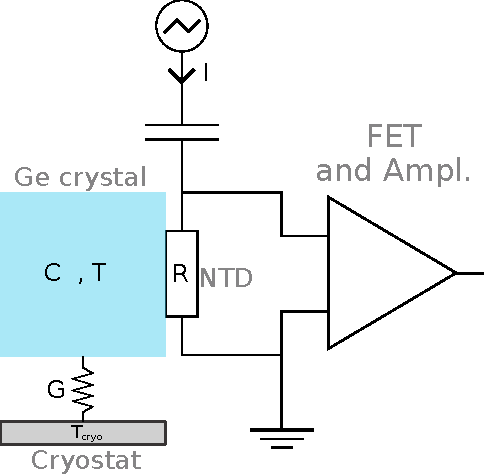
\includegraphics[width=0.3\textwidth]{graphics/bolo_simple.pdf}
\caption{\label{bolo-model} \em Simplified scheme of a RED bolometer coupling a thermal system (left side) and an electrical system (right side). }
\end{figure}

Here are some hints and info to help you understand the behavior of the bolometers (calculation and discussion in parallel with the measurements):
\begin{itemize}
	\item The heat power injected by the cryostat into the bolometer is $$P_{cryo} = G \left( T_{cryo} - T\right) \quad [\textrm{in } Watt]$$ In the considered simplified system, only the limiting conductance is considered (the lowest) which is generally the electron-phonon coupling (more in discussion..)
	\item A lot can be understand from studying the stationary state ($dT/dt=0$) and the time resolution (useful to introduce $\Delta T = T - T_{eq}$) of the heat equilibrium equation in the stationary state. Just recall that with $t$ the time and $U$ the energy of the thermal bath $$\frac{dU}{dt} = C \frac{dT}{dt} \quad [\textrm{in }  Joule]$$
	\item Some reference value for RED bolometers:
	$$ R = \mathcal{O}(1 \ G\Omega),\
	C \approx 3 \times 10^{-10} \ J.K^{-1},\
	G \approx 2 \times 10^{-8} \ W.K^{-1},\
	I = \mathcal{O}(1 \ nA),\
	T_{cryo} \approx 20 \ mK $$
	\item An optimized bolometer has the highest sensitivity $S_V$ in V/keV possible. Not to confuse with the sensitivity of the thermal sensor $\alpha$ which is usually introduced in this type of calculation 
	$$\alpha = \frac{1}{R} \frac{dR}{dT} $$
\end{itemize}


\subsection{Modélisation électrothermique du détecteur}

Dans cette partie, sont présenté les calculs théoriques permettant de construire le modèle du détecteur. L'étude s'est focalisée sur la résolution au premier ordre du système d'équations différentielles couplées en utilisant une méthode d'algèbre linéaire \cite{matrix}. Il est alors possible de simuler le comportement d'un détecteur dans l'état stationnaire, dans le régime temporel et dans le régime fréquentiel, ce qui donne accès à la caractérisation complète du détecteur.

\subsubsection{Description du modèle}

\begin{figure}[!ht]
%\centering
%\resizebox{0.6\textwidth}{!}{%
%\shorthandoff{:!}\begin{circuitikz}[scale=1]
%	%	\draw [help lines, step=0.5cm] (0.25,0) grid (7.75,5);
	\node [below] at (4, 0.05) {$T_b$};
	\fill [pattern = north east lines] (2.5,0.05) rectangle (5.5,0.25);
	\draw [brown, line width = 5] (4,0.25) -- (4,1.75);
	\draw [thick] (2.5,0.25) -- (5.5,0.25);
	\draw [brown, line width = 5] (3.25, 2.5) -- (1.75, 2.5);
	\draw [brown, line width = 5] (4.75, 2.5) -- (6.25, 2.5);
	\node [right] at (4, 1)	{$G_{pb}$};
	\node [left] at (4, 1)	{$P_{pb}$};
	\node [below] at (2.5, 2.5)	{$G_{ap}$};
	\node [above] at (2.5, 2.5)	{$P_{ap}$};
	\node [below] at (5.5, 2.5)	{$G_{ep}$};
	\node [above] at (5.5, 2.5)	{$P_{ep}$};
	\draw [fill=yellow] (3.25, 1.75) rectangle (4.75, 3.25);
	\node at (4, 2.5) {$T_p, C_p$};
	\draw [fill=orange] (1.75, 1.75) rectangle (0.25, 3.25);
	\node at (1, 2.5) {$T_a, C_a$};
	\draw [fill=cyan] (6.25, 1.75) rectangle (7.75, 3.25);
	\node at (7, 2.5) {$T_e, C_a$};
	\node [anchor=south, inner sep=0] at (1, 3.5)
    	{\resizebox{2cm}{!}{% This file was created by matplotlib2tikz v0.6.10.
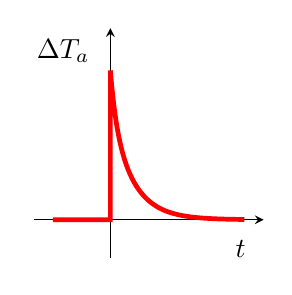
\begin{tikzpicture}

\begin{axis}[
ticks=none,
xmin=-0.2, xmax=0.4,
ymin=-0.5e-07, ymax=2.5e-07,
axis x line=center,
axis y line=center,
every axis x label/.style={at={(ticklabel cs:0.9)}, below=4pt},
every axis y label/.style={at={(ticklabel cs:0.9)}, left=4pt},
xlabel={$t$},
ylabel={$\Delta T_a$},
width=4.5cm,
height=4.5cm
]
\addplot [line width = 1.7pt, red]
table {%
-0.15 0
1e-08 0
0 1.94905773450583e-07
0.00353535353535354 1.75086151002447e-07
0.00707070707070707 1.58214334725911e-07
0.0106060606060606 1.4370498349366e-07
0.0141414141414141 1.31131841539708e-07
0.0176767676767677 1.20154073651191e-07
0.0212121212121212 1.10498558052284e-07
0.0247474747474747 1.01945886553252e-07
0.0282828282828283 9.43192935859211e-08
0.0318181818181818 8.74758993005682e-08
0.0353535353535354 8.1299781085828e-08
0.0388888888888889 7.56964899078769e-08
0.0424242424242424 7.05887084549368e-08
0.045959595959596 6.59128117256344e-08
0.0494949494949495 6.16161409749693e-08
0.053030303030303 5.76548416413408e-08
0.0565656565656566 5.39921472429897e-08
0.0601010101010101 5.05970160062528e-08
0.0636363636363636 4.74430465564955e-08
0.0671717171717172 4.45076144595586e-08
0.0707070707070707 4.17711836111647e-08
0.0742424242424242 3.92167561164711e-08
0.0777777777777778 3.68294319208594e-08
0.0813131313131313 3.45960554718693e-08
0.0848484848484848 3.25049314471608e-08
0.0883838383838384 3.05455953401098e-08
0.0919191919191919 2.8708627662862e-08
0.0954545454545454 2.69855028720667e-08
0.098989898989899 2.53684659759339e-08
0.102525252525253 2.38504312460595e-08
0.106060606060606 2.24248986152695e-08
0.10959595959596 2.10858842580303e-08
0.113131313131313 1.98278625736718e-08
0.116666666666667 1.86457173650087e-08
0.12020202020202 1.75347004576861e-08
0.123737373737374 1.64903963638234e-08
0.127272727272727 1.55086918770988e-08
0.130808080808081 1.45857497109756e-08
0.134343434343434 1.37179854696812e-08
0.137878787878788 1.29020473825878e-08
0.141414141414141 1.21347983445272e-08
0.144949494949495 1.14132998934018e-08
0.148484848484848 1.07347978270466e-08
0.152020202020202 1.00967092174591e-08
0.155555555555556 9.49661062525964e-09
0.159090909090909 8.93222735294378e-09
0.162626262626263 8.40142360402661e-09
0.166161616161616 7.9021934380375e-09
0.16969696969697 7.43265242968028e-09
0.173232323232323 6.99102995525483e-09
0.176767676767677 6.57566204137687e-09
0.18030303030303 6.18498472071477e-09
0.183838383838384 5.81752784734487e-09
0.187373737373737 5.4719093307749e-09
0.190909090909091 5.14682975298612e-09
0.194444444444444 4.84106733722839e-09
0.197979797979798 4.5534732409492e-09
0.201515151515152 4.28296714829148e-09
0.205050505050505 4.02853314017069e-09
0.208585858585859 3.78921582212947e-09
0.212121212121212 3.56411669204082e-09
0.215656565656566 3.35239073134553e-09
0.219191919191919 3.15324320491336e-09
0.222727272727273 2.96592665584594e-09
0.226262626262626 2.78973808262336e-09
0.22979797979798 2.62401628695844e-09
0.233333333333333 2.46813938158316e-09
0.236868686868687 2.32152244796522e-09
0.24040404040404 2.18361533465225e-09
0.243939393939394 2.05390058757701e-09
0.247474747474747 1.93189150423773e-09
0.251010101010101 1.81713030419968e-09
0.254545454545455 1.70918640885407e-09
0.258080808080808 1.6076548238223e-09
0.261616161616162 1.51215461781191e-09
0.265151515151515 1.42232749211878e-09
0.268686868686869 1.3378364353309e-09
0.272222222222222 1.2583644581251e-09
0.275757575757576 1.18361340336156e-09
0.279292929292929 1.11330282697358e-09
0.282828282828283 1.04716894542388e-09
0.286363636363636 9.84963645754594e-10
0.28989898989899 9.26453554498324e-10
0.293434343434343 8.71419161942022e-10
0.296969696969697 8.19653998446613e-10
0.30050505050505 7.70963859722854e-10
0.304040404040404 7.25166078149621e-10
0.307575757575758 6.82088837395062e-10
0.311111111111111 6.41570527764773e-10
0.314646464646465 6.03459139854875e-10
0.318181818181818 5.67611694232354e-10
0.321717171717172 5.33893705000791e-10
0.325252525252525 5.02178675237199e-10
0.328787878787879 4.72347622405636e-10
0.332323232323232 4.44288631966024e-10
0.335858585858586 4.17896437502591e-10
0.339393939393939 3.93072025796083e-10
0.342929292929293 3.69722265357532e-10
0.346464646464646 3.47759557029615e-10
0.35 3.27101505344391e-10
};
\end{axis}

\end{tikzpicture}}};
    \node [anchor=south, inner sep=0] at (4, 3.5)
    	{\resizebox{2cm}{!}{% This file was created by matplotlib2tikz v0.6.10.
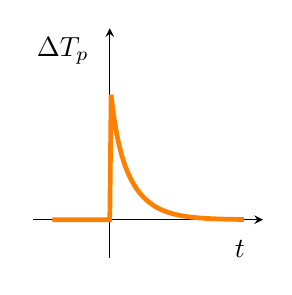
\begin{tikzpicture}

\definecolor{color0}{rgb}{1,0.647058823529412,0}


\begin{axis}[
ticks=none,
xmin=-0.2, xmax=0.4,
ymin=-0.5e-07, ymax=2.5e-07,
axis x line=center,
axis y line=center,
every axis x label/.style={at={(ticklabel cs:0.9)}, below=4pt},
every axis y label/.style={at={(ticklabel cs:0.9)}, left=4pt},
xlabel={$t$},
ylabel={$\Delta T_p$},
width=4.5cm,
height=4.5cm
]
\addplot [line width = 1.7pt, orange]
table {%
-0.15 0
1e-08 0
0 6.96368541805659e-24
0.00353535353535354 1.63176399143611e-07
0.00707070707070707 1.48010174769528e-07
0.0106060606060606 1.34895295323391e-07
0.0141414141414141 1.23468086776223e-07
0.0176767676767677 1.13437308330477e-07
0.0212121212121212 1.04569165237934e-07
0.0247474747474747 9.6675457798133e-08
0.0282828282828283 8.96042081124974e-08
0.0318181818181818 8.32322445633661e-08
0.0353535353535354 7.74593332500688e-08
0.0388888888888889 7.22035319129691e-08
0.0424242424242424 6.73975100378826e-08
0.045959595959596 6.29856326697683e-08
0.0494949494949495 5.89216479870297e-08
0.053030303030303 5.51668522742115e-08
0.0565656565656566 5.16886324595516e-08
0.0601010101010101 4.8459307338149e-08
0.0636363636363636 4.54552051530634e-08
0.0671717171717172 4.26559282807991e-08
0.0707070707070707 4.00437660952089e-08
0.0742424242424242 3.76032252420987e-08
0.0777777777777778 3.53206530016271e-08
0.0813131313131313 3.31839345070543e-08
0.0848484848484848 3.11822486108937e-08
0.0883838383838384 2.93058703676763e-08
0.0919191919191919 2.75460106137664e-08
0.0954545454545454 2.58946851090798e-08
0.098989898989899 2.43446072738405e-08
0.102525252525253 2.28890997930618e-08
0.106060606060606 2.15220213413162e-08
0.10959595959596 2.02377054550822e-08
0.113131313131313 1.90309091926043e-08
0.116666666666667 1.78967697058042e-08
0.12020202020202 1.68307672321937e-08
0.123737373737374 1.58286933182089e-08
0.127272727272727 1.48866233256637e-08
0.130808080808081 1.40008924633649e-08
0.134343434343434 1.31680747367947e-08
0.137878787878788 1.23849643284248e-08
0.141414141414141 1.16485590162039e-08
0.144949494949495 1.0956045313217e-08
0.148484848484848 1.0304785071529e-08
0.152020202020202 9.69230334102103e-09
0.155555555555556 9.11627731213953e-09
0.159090909090909 8.57452620193543e-09
0.162626262626263 8.06500196714538e-09
0.166161616161616 7.58578074763144e-09
0.16969696969697 7.13505495923382e-09
0.173232323232323 6.71112596779503e-09
0.176767676767677 6.31239728640301e-09
0.18030303030303 5.93736824626804e-09
0.183838383838384 5.58462809848333e-09
0.187373737373737 5.25285050953076e-09
0.190909090909091 4.94078841802559e-09
0.194444444444444 4.64726922404115e-09
0.197979797979798 4.37119028557055e-09
0.201515151515152 4.111514699389e-09
0.205050505050505 3.86726734587531e-09
0.208585858585859 3.63753117931072e-09
0.212121212121212 3.4214437468602e-09
0.215656565656566 3.21819392090423e-09
0.219191919191919 3.02701883066689e-09
0.222727272727273 2.84720098021137e-09
0.226262626262626 2.67806554087111e-09
0.22979797979798 2.51897780707433e-09
0.233333333333333 2.36934080531901e-09
0.236868686868687 2.2285930467763e-09
0.24040404040404 2.09620641465547e-09
0.243939393939394 1.97168417806043e-09
0.247474747474747 1.85455912461491e-09
0.251010101010101 1.74439180463596e-09
0.254545454545455 1.64076888009906e-09
0.258080808080808 1.54330157206693e-09
0.261616161616162 1.45162420065171e-09
0.265151515151515 1.36539281194944e-09
0.268686868686869 1.28428388672967e-09
0.272222222222222 1.20799312598366e-09
0.275757575757576 1.13623430873391e-09
0.279292929292929 1.06873821778733e-09
0.282828282828283 1.00525162937641e-09
0.286363636363636 9.45536362877567e-10
0.28989898989899 8.89368387025501e-10
0.293434343434343 8.36536979257968e-10
0.296969696969697 7.86843935027003e-10
0.30050505050505 7.4010282410245e-10
0.304040404040404 6.96138291071478e-10
0.307575757575758 6.54785397404927e-10
0.311111111111111 6.15889002618282e-10
0.314646464646465 5.79303182202572e-10
0.318181818181818 5.44890680139068e-10
0.321717171717172 5.12522393941935e-10
0.325252525252525 4.82076890295391e-10
0.328787878787879 4.53439949467044e-10
0.332323232323232 4.26504136787296e-10
0.335858585858586 4.01168399586413e-10
0.339393939393939 3.77337688076548e-10
0.342929292929293 3.5492259875595e-10
0.346464646464646 3.33839038997186e-10
0.35 3.14007911560752e-10
};
\end{axis}

\end{tikzpicture}}};	
    \node [anchor=south, inner sep=0] at (7, 3.5)
    	{\resizebox{2cm}{!}{% This file was created by matplotlib2tikz v0.6.10.
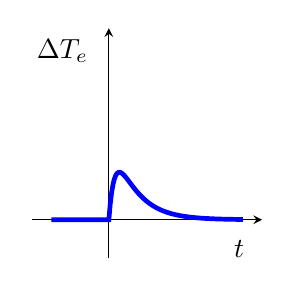
\begin{tikzpicture}

\begin{axis}[
ticks=none,
xmin=-0.2, xmax=0.4,
ymin=-0.5e-07, ymax=2.5e-07,
axis x line=center,
axis y line=center,
every axis x label/.style={at={(ticklabel cs:0.9)}, below=4pt},
every axis y label/.style={at={(ticklabel cs:0.9)}, left=4pt},
xlabel={$t$},
ylabel={$\Delta T_e$},
width=4.5cm,
height=4.5cm
]
\addplot [line width = 1.7pt, blue]
table {%
-0.15 0
1e-08 0
0 5.15986218822629e-23
0.00353535353535354 2.02319742455945e-08
0.00707070707070707 3.50283638973746e-08
0.0106060606060606 4.55829895717481e-08
0.0141414141414141 5.2854683483701e-08
0.0176767676767677 5.75967408445595e-08
0.0212121212121212 6.04003591661948e-08
0.0247474747474747 6.17289341324563e-08
0.0282828282828283 6.19451332621564e-08
0.0318181818181818 6.13322662511764e-08
0.0353535353535354 6.0111151566108e-08
0.0388888888888889 5.84534266690334e-08
0.0424242424242424 5.64920500734984e-08
0.045959595959596 5.4329586121974e-08
0.0494949494949495 5.20447391339915e-08
0.053030303030303 4.96975054505508e-08
0.0565656565656566 4.73332344043295e-08
0.0601010101010101 4.49858280406682e-08
0.0636363636363636 4.26802610766907e-08
0.0671717171717172 4.04345644105182e-08
0.0707070707070707 3.82613853431711e-08
0.0742424242424242 3.6169213865249e-08
0.0777777777777778 3.41633455563404e-08
0.0813131313131313 3.22466367949145e-08
0.0848484848484848 3.04200962489964e-08
0.0883838383838384 2.86833473567554e-08
0.0919191919191919 2.70349891927568e-08
0.0954545454545454 2.54728773405602e-08
0.098989898989899 2.39943418321705e-08
0.102525252525253 2.25963556141392e-08
0.106060606060606 2.12756641571379e-08
0.10959595959596 2.00288845812559e-08
0.113131313131313 1.88525808972803e-08
0.116666666666667 1.77433205654116e-08
0.12020202020202 1.66977164687768e-08
0.123737373737374 1.571245752772e-08
0.127272727272727 1.4784330493241e-08
0.130808080808081 1.39102349154358e-08
0.134343434343434 1.30871928548508e-08
0.137878787878788 1.23123545671688e-08
0.141414141414141 1.15830011255645e-08
0.144949494949495 1.0896544735358e-08
0.148484848484848 1.02505273303853e-08
0.152020202020202 9.64261791040749e-09
0.155555555555556 9.07060897650632e-09
0.159090909090909 8.53241234089511e-09
0.162626262626263 8.02605452431492e-09
0.166161616161616 7.54967190452406e-09
0.16969696969697 7.10150574045727e-09
0.173232323232323 6.67989716615275e-09
0.176767676767677 6.2832822247284e-09
0.18030303030303 5.91018699411838e-09
0.183838383838384 5.55922284183937e-09
0.187373737373737 5.2290818348624e-09
0.190909090909091 4.91853232202482e-09
0.194444444444444 4.62641469977975e-09
0.197979797979798 4.35163736701518e-09
0.201515151515152 4.09317287084003e-09
0.205050505050505 3.85005424236218e-09
0.208585858585859 3.62137151936202e-09
0.212121212121212 3.40626845122712e-09
0.215656565656566 3.20393938043e-09
0.219191919191919 3.01362629409614e-09
0.222727272727273 2.83461603874513e-09
0.226262626262626 2.66623769102869e-09
0.22979797979798 2.50786007718652e-09
0.233333333333333 2.35888943395577e-09
0.236868686868687 2.21876720377107e-09
0.24040404040404 2.08696795725728e-09
0.243939393939394 1.96299743622671e-09
0.247474747474747 1.84639071063342e-09
0.251010101010101 1.73671044319756e-09
0.254545454545455 1.63354525568494e-09
0.258080808080808 1.53650819110403e-09
0.261616161616162 1.44523526636046e-09
0.265151515151515 1.359384110183e-09
0.268686868686869 1.27863268140426e-09
0.272222222222222 1.20267806293949e-09
0.275757575757576 1.13123532705958e-09
0.279292929292929 1.06403646779599e-09
0.282828282828283 1.00082939654757e-09
0.286363636363636 9.41376997180387e-10
0.28989898989899 8.85456237122462e-10
0.293434343434343 8.32857331155583e-10
0.296969696969697 7.83382954796269e-10
0.30050505050505 7.36847504337837e-10
0.304040404040404 6.93076400795766e-10
0.307575757575758 6.51905435159421e-10
0.311111111111111 6.13180152505136e-10
0.314646464646465 5.76755272669063e-10
0.318181818181818 5.42494145313467e-10
0.321717171717172 5.10268237347692e-10
0.325252525252525 4.79956650785216e-10
0.328787878787879 4.51445669231489e-10
0.332323232323232 4.24628331303897e-10
0.335858585858586 3.9940402938568e-10
0.339393939393939 3.75678132210213e-10
0.342929292929293 3.53361629861074e-10
0.346464646464646 3.32370799857171e-10
0.35 3.12626893071057e-10
};
\end{axis}

\end{tikzpicture}}};
    	
%\end{circuitikz}\shorthandon{:!}
%}%
\begin{center}
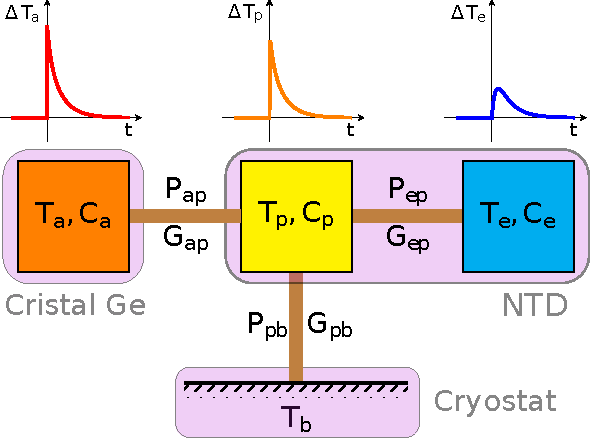
\includegraphics[width=0.6\textwidth]{Images/thermal_scheme.pdf}
\end{center}
\caption{Schéma thermique de RED1 et RED10 avec représentation de la diffusion d'un signal créée par un évènement dans le cristal de germanium. Chaque bain thermique est caractérisé par une température $T$ et une capacité thermique $C$. Chaque lien thermique est associé à une conductivité thermique $G$ et un transfert de puissance thermique $P$. Le senseur NTD est modélisé comme un système de phonons (index $p$) et un systèmes d'élécrons (index $e$) couplés thermiquement. Le bain absorbeur (index $a$) et  le cryostat (index $b$) sont tout deux reliés au bain de phonon du NTD. 
}
\label{thermal-scheme}
\end{figure}

\begin{figure}[!ht]
\begin{minipage}[c]{0.45\textwidth}
\resizebox{!}{\textwidth}{%
%\shorthandoff{:!}
\begin{circuitikz}[scale=1]
	  	\draw
	 (0.5,6) node [ground, rotate=-90] {} 
	 to [european voltage source, v=$V_B$, -*] (2,6)
	 to [european voltage source, l={\color{red} $e_{J_{RL}}$}, color=red] (2,4.5)	 
	 to [R, l_=$R_L$, -] (2,2.5)
	 to [thR, l_=$R(T_e)$, -] (2,0.5)
	 to [european voltage source, l={\color{red} $e_{J_{NTD}}$}, color=red]
	  (2,-0.5) node [ground] {}
	 (2,2.5) to [short, -o] (4,2.5) node [anchor=south] {$V$}
	 to [C, l_=$C_{fil}$] (4,-0.5) node [ground] {} 
	 (4,2.5) to [european voltage source, l={\color{red} $e_{ampli.}$}, color=red] (6,2.5) 
	 to [ioosource, l={\color{red} $i_{ampli.}$}, color=red] (6,-0.5) node [ground] {} 
	 (6,2.5) node [anchor=south] {$U$}
	 to [short, i_={\small $i \approx 0$}, *-] (7,2.5)
	 to [amp, l=Suiveur, -] (8,2.5)
	;
\end{circuitikz}
%\shorthandon{:!}
}%
\end{minipage}
\hfill
\vrule{}
\hfill
\begin{minipage}[c]{0.45\textwidth}
\begin{center}
avec Thèvenin-Norton, en fréquentiel :
\end{center}
\resizebox{\textwidth}{!}{%
%\shorthandoff{:!}
\begin{circuitikz}
		\draw
	 (0,0) node [ground] {}
	 to [R, l_=$Z_{eq}$, -] (0,2)
	 (0,2) to [short, -o] (2,2) node [anchor=south] {$V$}
	 to [ioosource, l=$\color{red} i_{bruit}$,color=red, -] 
	 (2,0) node [ground] {}
	 (2,2) to [european voltage source, l={\color{red} $e_{ampli.}$}, color=red, -] (4,2) node [anchor=south] {$U$}
	 to [short, i_={\small $i \approx 0$}, *-] (5,2)
	 to [amp, l=Suiveur, -] (6,2)
	 (0,-1.5) node [right]{$\color{red} \displaystyle i_{bruit}^2=\left(\frac{e_{J_{NTD}}}{R(T_e)}\right)^2+\left(\frac{e_{J_{R_L}}}{R_L}\right)^2+i_{ampli.}^2$}
	;
\end{circuitikz}
%\shorthandon{:!}
}%
\end{minipage}
\caption{Schémas de l'électronique de polarisation. La résistance NTD $R(T_e)$, la résistance de charge $R_L$ et la capacité du câblage $C_{fil}$ deviennent l'impédance complexe équivalente $Z_{eq}$. Les sources de bruits apparaissent en rouge. Les bruits Johnson, $e_{J_{RL}}$ et $e_{J_{NTD}}$, ainsi que le bruit en courant de l'amplificateur $i_{ampli.}$ sont regroupés en un bruit en courant $i_{bruit}$ dont l'expression est précisée.}
\label{electric-scheme}
\end{figure}

On utilise l'approximation d'un système de trois bains thermiques pour modéliser un détecteur RED \cite{note}. Le schéma thermique d'un détecteur dans une telle approximation est présenté dans la \hyperref[thermal-scheme]{Figure 1}. Ce modèle modélise au mieux \cite{albert} \cite{benjamin} un absorbeur en cristal de germanium sur lequel est collé un unique senseur thermique NTD. Comme présenté sur la \hyperref[thermal-scheme]{Figure 1}, il y a trois bains thermiques, chacun caractérisé par une capacité thermique $C$ et une température $T$ :
\begin{itemize}
\item en orange, le cristal de germanium jouant le rôle d'absorbeur ($T_a$, $C_a$),
\item en jaune, le bain thermique des phonons dans la résistance NTD ($T_p$, $C_p$),
\item en bleu, le bain thermique des électrons dans la résistance NTD ($T_e$, $C_e$).
\end{itemize}
Ils sont reliés par des liens thermiques caractérisés par des conductivités thermiques $G$, ce qui permet un transfert de puissance $P$ entre les bains. Il y a également la présence d'une fuite thermique de la résistance NTD vers le cryostat (en tirets noirs) ce qui permet de fixer une température de fonctionnement $T_b$.
Afin de mesurer la variation de résistance du NTD, engendrée par un dépôt d'énergie au sein du détecteur lors d'une interaction avec une particule, il est nécessaire de polariser le senseur en courant. Cela se fait en ajoutant une résistance de charge très élevée en série. Le senseur NTD est alors parcouru par un courant de polarisation $I_P$ quasiment constant pendant un évènement \cite{elec}. Le schéma électronique qui permet la polarisation et la mesure de la tension $V$ aux bornes de la résistance NTD est présenté sur la figure \ref{electric-scheme}. Il y a à gauche le schéma de l'électronique de polarisation avec représentation des bruits (en rouge) et à droite la simplification du schéma par transformation de Thèvenin-Norton \cite{mather} dans le cadre de l'étude fréquentielle, qui viendra plus tard. Une tension de polarisation constante $V_B$ est appliquée à la résistance de charge $R_L$, de quelques $G\Omega$, en série avec la résistance du NTD $R(T_e)$ dépendante de la température du bain d'électrons. On tient compte de la capacité du câblage $C_{fil}$ de l'électronique.

Afin de prédire la réponse du détecteur à un évènement, il faut maintenant résoudre ce modèle électro-thermique. On définit alors le système d'équations différentielles couplées par l'échange de puissance entre les bains thermiques, et avec le système électronique par la puissance Joule induite par le courant de polarisation au sein du senseur NTD.

Pour le système d'électrons du NTD, on a d'abord une puissance provenant de l'effet Joule $P_J= I_P^2 R(T_e)=\frac{V^2}{R(T_e)}$. On a ensuite le transfert de puissance provenant du système phonons du NTD s'exprimant comme : $P_{ep}=V_{NTD} g_{ep} (T_e^n - T_p^n)$ où $V_{NTD}$ est le volume du senseur NTD, $g_{ep}$ est la constante de couplage électron-phonon par unité de volume et $n$ est un exposant dépendant du matériau qui vaut typiquement 6 pour les thermistors tel que les NTD en germanium. L'équation d'équilibre thermique pour le bain électrons est,
\begin{equation}
\label{electron}
 C_e \frac{d T_e}{d t} = \frac{V^2}{R(T_e)} - V_S g_{ep} \left( T_e^{n} - T_p^{n} \right)
\end{equation}

Pour l'absorbeur, le bain thermique représente uniquement le système de phonons du cristal de germanium. Ce matériau étant semi-conducteur sous forme de cristal ultra-pur, il n'existe pas d'électrons libres. L'absorbeur échange une puissance  avec le système de phonons du NTD en considérant la capacité thermique de la colle comme étant négligeable. Celle-ci s'écrit $P_{ap}=g_{glue} S_{NTD} \left( T_p^{n_g} - T_a^{n_g} \right)$ avec $S_{NTD}$ la surface du NTD collé sur l'absorbeur, $g_{glue}$ la constante de conductivité thermique par unité de surface et $n_g$ un exposant. Ces deux paramètres ont été fixé expérimentalement lors d'études précédentes. L'équation d'équilibre thermique pour ce bain est donc,
\begin{equation}
\label{absorbeur}
C_a \frac{d T_a}{d t} = g_{glue} S_{NTD} \left( T_p^{n_g} - T_a^{n_g} \right)
\end{equation}


Pour le système de phonons du NTD, on a la puissance provenant du couplage phonon-électron $P_{ep}$, le transfert de puissance provenant du cristal de germanium $P_{ap}$, et la fuite thermique d'or vers le cryostat. Cette conduction thermique est assurée par deux surfaces d'or $S_{Au}$ (une sur le NTD, une sur le support) reliées par des fils d'or. On a affaire à un processus non-diffusif appelé conduction Kapitza qui s'exprime : $P_{pb}=S_{Au} g_k (T_p^{n_k} - T_b^{n_k})$ avec $g_k$ la conductance Kapitza par unité de surface et l'exposant $n_k=4$. On néglige cette fois la capacité thermique des surfaces et fils d'or, tout en considérant une capacité thermique du support en cuivre infinie, permettant de garder une température fixe $T_b$ à tout temps.
Ce bain est décrit par l'équation :
\begin{equation}
\label{phonon}
C_p \frac{d T_p}{d t} = -g_{glue} S_{NTD} \left( T_p^{n_g} - T_a^{n_g} \right)  + V_S g_{ep} \left( T_e^{n} - T_p^{n} \right) - g_k S_{Au} \left( T_p^{n_k} - T_b^{n_k} \right)
\end{equation}

Le système électrique prend en compte la variation du courant de polarisation (effet du second ordre sir $R_L\ll R_{NTD}$). L'équation associée est,
\begin{equation}
\label{polarisation}
C_{fil} \frac{d V}{d t} = \frac{V_B - V}{R_L} - \frac{V}{R(T_e)}
\end{equation}

En rassemblant les équations \ref{electron}, \ref{absorbeur}, \ref{phonon} et \ref{polarisation}, on peut composer un système d'équations différentielles couplées qui décrit complètement le modèle électro-thermique présenté dans les figures \ref{thermal-scheme} et \ref{electric-scheme}.

\begin{align}
\label{ode}
 C_a \frac{d T_a}{d t} &= g_{glue} S_{NTD} \left( T_p^{n_g} - T_a^{n_g} \right) \nonumber \\ 
 C_p \frac{d T_p}{d t} &= -g_{glue} S_{NTD} \left( T_p^{n_g} - T_a^{n_g} \right)  + V_S g_{ep} \left( T_e^{n} - T_p^{n} \right) - g_k S_{Au} \left( T_p^{n_k} - T_b^{n_k} \right) \nonumber \\ 
 C_e \frac{d T_e}{d t} &= \frac{V^2}{R(T_e)} - V_S g_{ep} \left( T_e^{n} - T_p^{n} \right) \nonumber \\ 
 C_{fil} \frac{d V}{d t} &= \frac{V_B - V}{R_L} - \frac{V}{R(T_e)}
\end{align}

\subsubsection{Solution de l'état stationnaire}
\label{steady-section}

L'étude de l'état stationnaire permet d'obtenir les grandeurs physiques autour desquels les perturbations du système vont se produire. Il est essentiel de le calculer pour obtenir les valeurs de résistance NTD, des capacités thermiques et des conductivité thermiques. Il est également nécessaire pour effectuer une opération de linéarisation par la suite. L'état stationnaire est expérimentalement défini par la température du cryostat $T_b$ et le courant de polarisation $I_P$. 

Il suffit d'annuler les termes de dérivées temporelles dans le système d'équations (\ref{ode}) pour obtenir le système d'équations dans l'état stationnaire avec ($\bar{T}_a, \bar{T}_p, \bar{T}_e, \bar{V}$) étant les solutions de l'état stationnaire :
\begin{align}
\label{steady}
0 &= g_{glue} S_{NTD} \left( \bar{T}_p^{n_g} - \bar{T}_a^{n_g} \right) \nonumber \\
0 &= -g_{glue} S_{NTD} \left( \bar{T}_p^{n_g} - \bar{T}_a^{n_g} \right) + V_S  g_{ep} \left( \bar{T}_e^{n} - \bar{T}_p^{n} \right) - g_k S_{Au} \left( \bar{T}_p^{n_k} - \bar{T}_b^{n_k} \right) \nonumber \\
0 &= \frac{V^2}{R(\bar{T}_e)} - V_S g_{ep} \left( \bar{T}_e^{n} - \bar{T}_p^{n} \right) \nonumber \\
0 &= \frac{V_B - V}{R_L} - \frac{V}{R(\bar{T}_e)}
\end{align}

Les équations sont non linéaires de part l'expression des puissances échangées et de la résistance NTD. Il est nécessaire d'employer une résolution numérique pour résoudre ce système. 


\subsubsection{Comportement dans le domaine temporel}
\label{temporal}


La résolution du système d'équations (\ref{ode}) donnerait les expressions exactes de l'évolution temporelle des températures des différents bains $T_a(t), T_p(t), T_e(t)$ et de la tension aux bornes du NTD $V(t)$. Toutefois, la très forte non-linéarité du système ne permet pas une résolution analytique. Néanmoins, seule la réponse du système à un évènement nous intéresse. L'énergie déposée d'environ $1$keV par une particule dans l'absorbeur s'exprime comme une élévation de température de l'ordre de $100~\mu K$, ce qui donne une variation de tension aux bornes du NTD de l'ordre de $100~nV$. Il est ainsi question d'étudier la réponse du système à de très faibles signaux. On se propose d'appliquer une théorie perturbative au premier ordre au système d'équations (\ref{ode}). Avec la linéarisation des termes, il est possible de définir des conductivités thermiques pour les différents liens :
\begin{itemize}
\item colle cristal-NTD : \begin{equation}\label{g1} G_{ap}^a  = n_g g_{glue} S_{NTD} \bar{T}_a^{n_g-1} \qquad \textrm{et} \qquad G_{ap}^p  = n_g g_{glue} S_{NTD} \bar{T}_p^{n_g-1}
\end{equation}
\item couplage électrons-phonons : \begin{equation}\label{g2} G_{ep}^e  = n g_{ep} V_S \bar{T}_e^{n-1} \qquad \textrm{et} \qquad G_{ep}^p  = n g_{ep} V_S \bar{T}_p^{n-1}
\end{equation}
\item fuite thermique avec fils d'or : \begin{equation}\label{g3} G_{pb} = n_k g_{k} S_{Au} \bar{T}_p^{n_k-1}
\end{equation}
\end{itemize}
On remarquera que les conductivités ont un "sens" d'utilisation comme elles dépendent de la température des bains. En retranchant (\ref{ode}), on obtient alors un système d'équations linéaires couplées :
\begin{align}
\label{tempo}
C_a \frac{d \Delta T_a}{d t}
	&= -G_{ap}^a \Delta T_a + G_{ap}^p \Delta T_p 
	\nonumber \\
C_p \frac{d \Delta T_p}{d t} 
	&= +G_{ap}^a \Delta T_a - G_{ap}^p \Delta T_p
	+ G_{ep}^e \Delta T_e - G_{ep}^p \Delta T_p
	- G_{pb}^p \Delta T_p
	\nonumber \\
C_e \frac{d \Delta T_e}{d t}
	&= - G_{ep}^e \Delta T_e + G_{ep}^p \Delta T_p
	+2\frac{\bar{V}}{R(\bar{T}_e)} \Delta V - \frac{\bar{V}^2}{R(\bar{T}_e)^2} \left.\frac{d R}{d T}\right\vert_{T_e} \Delta T_e
 	\nonumber \\
C_{fil} \frac{d \Delta V}{d t} &= - \left( \frac{1}{R_L} + \frac{1}{R(\bar{T}_e)} \right) \Delta V + \frac{\bar{V}}{R(\bar{T}_e)^2} \left.\frac{d R}{d T}\right\vert_{\bar{T}_e} \Delta T_e
\end{align}
Celui-ci peut se simplifier :
\begin{align}
\label{tempo-bis}
\frac{d \Delta T_a}{d t}
	&= -\frac{G_{ap}^a}{C_a} \Delta T_a + \frac{G_{ap}^p}{C_a} \Delta T_p 
	\nonumber \\
\frac{d \Delta T_p}{d t} 
	&= \frac{G_{ap}^a}{C_p} \Delta T_a - \frac{G_{ap}^p+G_{ep}^p+G_{pb}^p}{C_p} \Delta T_p	+ \frac{G_{ep}^e }{C_p}\Delta T_e
	\nonumber \\
\frac{d \Delta T_e}{d t}
	&= \frac{G_{ep}^p}{C_e} \Delta T_p - \frac{1}{C_e} \left(G_{ep}^e + \frac{\bar{V}^2}{R(\bar{T}_e)^2} \left.\frac{d R}{d T}\right\vert_{\bar{T}_e}\right) \Delta T_e 
	+2 \frac{1}{C_e} \frac{\bar{V}}{R(\bar{T}_e)} \Delta V
 	\nonumber \\
\frac{d \Delta V}{d t} &= \frac{1}{C_{fil}} \frac{\bar{V}}{R(\bar{T}_e)^2} \left.\frac{d R}{d T}\right\vert_{\bar{T}_e} \Delta T_e - \frac{1}{C_{fil}}\left( \frac{1}{R_L} + \frac{1}{R(\bar{T}_e)} \right) \Delta V 
\end{align}
On étudie désormais un système d'équations linéaires. Il est ainsi possible de les résoudre analytiquement. Pour cela, on peut réécrire ce système d'équations sous forme matricielle afin de faciliter les calculs. On introduit le vecteur $\bm{\phi}$ contenant les perturbations de températures et de la tension :
\begin{equation}
\label{phi}
\bm{\phi} = 
\left( \begin{array}{c}
\Delta T_a\\
\Delta T_p\\
\Delta T_e\\
\Delta V
\end{array} \right)
\end{equation}
Le système (\ref{tempo-bis}) devient simplement :
\begin{equation}
\label{ode-mat}
\frac{d \bm{\phi}}{d t}= - \bm{M} \bm{\phi} + \bm{F}(t-t_0)
\end{equation}
où $\bm{M}$ est la matrice regroupant les termes de couplages életro-thermiques. Elle découle directement des équations précédentes (\ref{tempo-bis}), et s'exprime :
\begin{equation}
\label{coupling-mat-temp}
\bm{M} = 
\left( \begin{array}{cccc}
 \frac{G_{ap}^a}{C_a}&-\frac{G_{ap}^p}{C_a}&0&0 \\
 -\frac{G_{ap}^a}{C_p}&\frac{G_{ap}^p+G_{ep}^p+G_{pb}^p}{C_p}&-\frac{G_{ep}^e}{C_p}&0 \\
0&-\frac{G_{ep}^p}{C_e}&\frac{1}{C_e}\left(G_{ep}^e + \frac{V^2}{R(T_e)^2}  \left.\frac{d R}{d T}\right\vert_{T_e} \right)&-2\frac{V}{R(T_e)}\\
0&0&-\frac{1}{C_{fil}}\frac{V}{R(T_e)^2} \left.\frac{d R}{d T}\right\vert_{T_e} &\frac{1}{C_{fil}}\left( \frac{1}{R_L} + \frac{1}{R(T_e)} \right)
\end{array} \right)
\end{equation}
Il a également été ajouté un terme de source $\bm{F}$ qui permet de contenir les dépôts d'énergie dans le détecteur et les différentes sources de bruits parasites. Dans le cas d'une particule déposant une énergie $E$ dans l'absorbeur, ce terme s'exprime comme,
\begin{equation}
\bm{F}(t-t_0) = 
\left( \begin{array}{c}
E/C_a \\
0 \\
0 \\
0
\end{array} \right) \delta (t-t0)
\end{equation}
On considère ici le dépôt de l'énergie de recul, la relaxation des phonons créés dans l'absorbeur, et l'élévation en température de celui-ci comme étant des processus instantanés, d'où l'utilisation de la fonction de Dirac $\delta (t-t_0)$. Une variante de ce modèle consiste à attribuer un temps de relaxation aux phonons et de prendre en compte la montée en température des bains thermiques lors de la relaxation des phonons.

La solution générale de l'équation (\ref{ode-mat}) est une combinaison linéaire de $N$ exponentielles, avec $N=4$ correspondant aux dimensions du système, chacune étant caractérisée par une constante de temps. On obtient leur expression en diagonalisant la matrice de couplage $\bm{M}$ pour se placer dans la base propre des solutions du système. On considère, pour $i=1,2,3,4$, les vecteurs propres $\bm{v}_i$ et les valeurs propres associées pour écrire ces solutions,
\begin{equation}
\label{eigen-soluc}
\bm{f}_i(t) = f_i(t) \bm{v}_i
\end{equation}
Sans considérer le terme de source, on introduit ces expressions dans l'équation matricielle (\ref{ode-mat}) pour donner
\begin{equation}
\label{eigen-soluc-ode}
\frac{d \bm{f}_i(t)}{d t} = -f_i(t) \bm{M} \bm{v}_i = -\lambda_i f_i(t) \bm{v}_i
\end{equation}
La résolution de cette équation amène à l'expression des solutions dans la base propre $f_i(t) = A_i e^{-t/\tau_i} \bm{v}_i$ avec $A_i$ la constante de normalisation et $\tau_i=1/\lambda_i$ la constante de temps de la solution. La solution générale de (\ref{ode-mat}) s'exprime alors dans la base propre comme
\begin{equation}
\label{eigein-solc-expr}
\bm{f}(t) = \sum_i A_i e^{-t/\tau_i} \bm{v}_i
\end{equation}
Pour faire le lien entre la base propre et les fluctuations de températures et de tension, il faut projeter la solution $\bm{f}$ sur les 4 vecteurs orthogonaux formant $\bm{\phi}$ tel que :
\begin{equation}
\label{gen-soluc}
\phi_j = \bm{f} \cdot \bm{\phi}_j = \sum_i^4 f_i(t) \bm{v}_i \cdot \bm{\phi}_j = \sum_i P_{ij} f_i(t) = \sum_i P_{ij} A_i e^{-t/\tau_i}
\end{equation}
où $P_{ij}$ désigne les vecteurs composant la matrice de passage satisfaisant $\bm{M}=\bm{P} \bm{D} \bm{P}^{-1}$.

Pour fixer les constantes de normalisation $A_i$, on utilise les conditions initiales du système :
\begin{equation}
\bm{\phi}(0) = \bm{F}(0) =
\left( \begin{array}{c}
\sum_i P_{ai} A_i\\
\sum_i P_{pi} A_i\\
\sum_i P_{ei} A_i\\
\sum_i P_{vi} A_i
\end{array} \right) = \bm{P} \bm{A}
\qquad \longrightarrow \qquad \bm{A}=\bm{P}^{-1} \bm{\phi} (0)
\label{normal}
\end{equation}
avec $\bm{A}$ le vecteur contenant les constantes $A_i$.

L'étude d'un détecteur en temporel revient à résoudre l'équation matricielle (\ref{ode-mat}) et donc à trouver les valeurs et vecteurs propres de la matrice de couplage $\bm{M}$. Le modèle électro-thermique est maintenant complètement décrit dans le domaine temporel.

\subsubsection{Réponse en domaine fréquentiel}
\label{omega}

L'étude des bruits menant au calcul de la résolution du détecteur nécessite de décrire maintenant le comportement en régime fréquentiel. En effet, les bruits d'un système sont bien caractérisés d'un point de vue fréquentiel : on peut avoir accès à l'expression de leur densité spectrale.
On considère la transformée de Fourier de l'équation matricielle (\ref{ode-mat}),
\begin{equation}
\bm{C} (i\omega + \bm{M})  \bm{\tilde{\phi}}  (\omega) = \bm{Z} (\omega) \bm{\tilde{\phi}} (\omega)  = \bm{C} \bm{\tilde{F}} (\omega) \qquad \textrm{avec} \qquad \bm{C} = \left( \begin{array}{cccc}
 C_a&0&0&0 \\
0&C_p&0&0\\
0&0&C_e&0\\
0&0&0&C_{fil}
\end{array} \right)
\end{equation}
où l'on introduit une matrice $\bm{Z}$ contenant les couplages électro-thermiques exprimés dans le régime fréquentiel. En explicitant cette équation :
\begin{equation}
\label{z-mat}
\bm{Z} (\omega) \bm{\tilde{\phi}} (\omega) =
\left( \begin{array}{cccc}
 \frac{1}{a}&-g&0&0 \\
-b&\frac{1}{c}&-h&0\\
0&-d&\frac{1}{e}-k&-l\\
0&0&-f&Z_{eq}^{-1}
\end{array} \right)
\left( \begin{array}{c}
\Delta T_a\\
\Delta T_p\\
\Delta T_e\\
\Delta V
\end{array} \right)
 =
\left( \begin{array}{c}
W\begingroup\color{red} - P_{ap}\endgroup\\
\begingroup\color{red}  P_{ap} + P_{ep} + P_{bp}\endgroup\\
\begingroup\color{red} - P_{ep}\endgroup\\
\begingroup\color{red}  i_{bruit} \endgroup
\end{array} \right)
=  \bm{C} \bm{\tilde{F}} (\omega)
\end{equation}
avec les termes rouges étant des bruits en puissance et en courant introduits dans le diagramme en blocs \ref{block-diagram}. Les coefficients de la matrice $\bm{Z}$ découlent du système d'équations linéarisées (\ref{ode}) tels que :
\begin{equation}
\begin{aligned}[c]
a &=(i C_a \omega + G_{ap}^a)^{-1} \\
b &=G_{ap}^a \\
c &=(i C_p \omega + G_{ap}^p + G_{ep}^p + G_{pb})^{-1} \\
d &=G_{ep}^p \\
e &=(i C_e \omega + G_{ep}^e)^{-1}\\
f &=\frac{(dR/dT) V}{R^2} 
\end{aligned}
\qquad \qquad
\begin{aligned}[c]
g &=G_{ap}^p \\
h &=G_{ep}^e \\
k &=- \frac{(dR/dT) V^{2}}{R^{2}} \\
\ell &=\frac{2 V}{R}
\end{aligned}
\label{coef}
\end{equation}
et avec l'impédance complexe $Z_{eq}$ contenant les composants électriques du circuit de polarisation conformément à la figure (\ref{electric-scheme}) :
\begin{equation}
Z_{eq} = \left(\frac{1}{R_L} + \frac{1}{R(T_e)} + i\omega C_{fil}\right)^{-1}
\end{equation}
L'expression du vecteurs des fluctuations $\bm{\phi}$ s'obtient en inversant la matrice couplage $\bm{Z}$ comme, 
\begin{equation}
\bm{\tilde{\phi}} (\omega) =
\left( \begin{array}{c}
\Delta \tilde{T}_a\\
\Delta \tilde{T}_p\\
\Delta \tilde{T}_e\\
\Delta \tilde{V}
\end{array} \right)
=
\left( \begin{array}{cccc}
 Z_{aa}^{-1}&Z_{ap}^{-1}&Z_{ae}^{-1}&Z_{av}^{-1} \\
 Z_{pa}^{-1}&Z_{pp}^{-1}&Z_{pe}^{-1}&Z_{pv}^{-1}\\
 Z_{ea}^{-1}&Z_{ep}^{-1}&Z_{ee}^{-1}&Z_{ev}^{-1}\\
 Z_{va}^{-1}&Z_{vp}^{-1}&Z_{ve}^{-1}&Z_{vv}^{-1}
\end{array} \right)
\left( \begin{array}{c}
\Delta \tilde{P}_a\\
\Delta \tilde{P}_p\\
\Delta \tilde{P}_e\\
\Delta \tilde{I}
\end{array} \right)
= \bm{Z}^{-1}(\omega) \bm{\tilde{F}} (\omega)
\end{equation}
On remarque ici que le formalisme matriciel associé à un outil de calcul numérique permet d'avoir facilement accès aux perturbations de températures et de tension à partir de la matrice de couplage et des sources de puissances externes contenues dans le vecteur $\bm{\tilde{F}}(w)$.

\begin{figure}[!ht]
\begin{center}
\resizebox{\textwidth}{!}{%
\begin{tikzpicture}
	    \sbEntree{W}
    \sbCompSum{C1}{W}{-}{+}{+}{}
    	\sbRelier{W}{C1}
        \sbNomLien[0.8]{W}{$W$}
    \sbBloc{a}{$a$}{C1}
        \sbRelier{C1}{a}
    \sbBloc[3]{b}{$b$}{a}
        \sbRelier[$\Delta T_a$]{a}{b}  
    \sbCompSum{C2}{b}{+}{+}{+}{}
        \sbRelier{b}{C2}      
    \sbBlocL{c}{$c$}{C2}
    \sbBloc[3]{d}{$d$}{c}
    	\sbRelier[$\Delta T_p$]{c}{d}
    \sbCompSum{C3}{d}{-}{+}{+}{}
    	\sbRelier{d}{C3}		
    \sbBlocL{e}{$e$}{C3}	      
    \sbBloc[3]{f}{$f$}{e}
    	\sbRelier[$\Delta T_e$]{e}{f}
    \sbCompSum{C4}{f}{+}{}{+}{}
        \sbRelier{f}{C4}
    \sbBlocL{Z}{$Z_{eq}$}{C4}
    \sbCompSum[5]{C5}{Z}{+}{}{+}{}
        \sbRelier[$\Delta U$]{Z}{C5}
    \sbSortie{V}{C5}
        \sbRelier{C5}{V}
        \sbNomLien[0.8]{V}{$\Delta V$}
    
    \sbDecaleNoeudy[5]{a-b}{down1}
	\sbBlocr{g}{$g$}{down1}
		\sbRelieryx{c-d}{g}
    	\sbRelierxy{g}{C1}
    \sbDecaleNoeudy[8]{c-d}{down2}
	\sbBlocr{h}{$h$}{down2}
		\sbRelieryx{e-f}{h}
    	\sbRelierxy{h}{C2}
	\sbDecaleNoeudy[10]{d}{down5}
	\sbCompSum{C6}{down5}{}{+}{}{+}
	\sbBloc{k}{$k$}{C6}
	\sbDecaleNoeudy[13]{C4-Z}{down4}
	\sbBlocr{l}{$\ell$}{down4}
		\sbRelier[$\Delta P_J$]{C6}{C3}
		\sbRelieryx{e-f}{k}
    	\sbRelier{k}{C6}	
		\sbRelieryx{Z-C5}{l}
    	\sbRelierxy{l}{C6}
    
    \sbStyleLien{red,text=red}
    \sbDecaleNoeudy[-4]{C1}{Pap}
    	\sbRelier{Pap}{C1}
    	\sbNomLienCustom[0.3]{Pap}{$P_{ap}$}
    \sbDecaleNoeudy[-4]{C2}{sumP}
    	\sbRelier{sumP}{C2}
    	\sbNomLienCustom[0.3]{sumP}{$P_{ap}+P_{ep}+P_{bp}$}
    \sbDecaleNoeudy[-4]{C3}{Pep}
    	\sbRelier{Pep}{C3}
    	\sbNomLienCustom[0.3]{Pep}{$P_{ep}$}
    \sbDecaleNoeudy[-4]{C4}{i}
    	\sbRelier{i}{C4}
    	\sbNomLienCustom[0.3]{i}{$i_{bruit}$}  
    \sbDecaleNoeudy[-3]{C5}{eA}
    	\sbRelier{eA}{C5}
    	\sbNomLienCustom[0.3]{eA}{$e_{ampli.}$}   
\end{tikzpicture}
}%
\end{center}
\caption{Diagramme en bloc du modèle électro-thermique avec injection de la puissance d'un évènement $W$, de bruits en puissance $P_{ap}, P_{ep}, P_{pb}$, d'un bruit en courant $i_{bruit}$ et d'un bruit en tension $e_{ampli.}$. Les coefficients des blocs sont précisés dans (\ref{coef}). Le formalisme des diagrammes en blocs et le formalisme matricielle sont équivalents et aboutissent à des expressions identiques pour les calculs de sensibilité et de bruit.}
\label{block-diagram}
\end{figure}

Malgré cette simplification des calculs, la compréhension des couplages entre les grandeurs observées n'est pas très aisée. Une meilleure compréhension est possible en convertissant le système d'équations (\ref{ode-mat}) dans un formalisme de diagramme en blocs \cite{block-diagram} présenté à la figure \ref{block-diagram}. On y retrouve les coefficients de couplages utilisés dans la matrice de couplage $\bm{Z}$ ainsi que les sources de puissances externes. On peut visualiser plus aisément le couplage entre les différents bains ainsi que la diffusion de la puissance déposée par une particule dans l'absorbeur $W$.

La réponse du système à un évènement est caractérisée par la sensibilité $s_V$. Dans le cas d'une interaction de particule déposant toute l'énergie de recul dans l'absorbeur, la sensibilité s'exprime ${s}_V(\omega) = Z_{va}^{-1}\hat{p}(\omega)$ avec $\hat{p}(\omega)$ la transformée de Fourier du signal en puissance $W$. L'approximation d'un dépôt d'énergie de recul instantané donne $\hat{p}(\omega) = \hat{\delta} = 1$, ce qui simplifie énormément les calculs. La variante où l'on considère le temps de relaxation des phonons nécessite de multiplier par la fonction passe-bas $\hat{p}(\omega) = 1/(1+i\omega \tau_P)$ avec $\tau_P$ la constante de temps correspondant au temps de relaxation des phonons au sein du détecteur. D'autres expériences de détection directe, telles que CDMS \cite{julien}, travaillent par la détection des phonons athermaux qui traverseraient les différentes parties du détecteur avant de se relaxer. Ainsi, il est possible d'avoir une fraction $\epsilon$ des phonons, produit lors d'un évènement, qui passe dans la résistance NTD et s'y relaxent. On observerait alors une élévation de température directement dans le senseur NTD, en plus de celle dans l'absorbeur. En prenant en compte cette possiblité, la sensibilité du système se réécrit :
\begin{equation}
\label{sv}
\hat{s}_V(\omega) = \left[(1-\epsilon) Z_{va}^{-1} + \epsilon Z_{ve}^{-1}\right]\hat{p}(\omega) \qquad [V/W]
\end{equation}
La fraction $\epsilon$ de phonons dits "athermiques" dépend très fortement de la géométrie du cristal de germanium, de son polissage, de la colle utilisée entre l'absorbeur et le NTD, et sûrement d'autres paramètres de l'expérience qui ne sont pas encore cernés. On détecte la présence de phonons athermiques grâce à la forme du signal : la montée en température du NTD est plus rapide et il apparait une contribution exponentielle caractérisée par la constante de temps $\tau_P$. On verra dans les parties suivantes que le détecteur RED10 présente une fraction importante de phonons athermiques qui est estimée par la forme du signal.

La résolution du diagramme en bloc \ref{block-diagram} permet de s'assurer que la boucle de rétro-action associée à la puissance Joule $\Delta P_J$ est négative, ce qui permet la stabilité de la polarisation de la résistance NTD. En effet, l'élévation en température créée par le courant de polarisation dans le NTD diminue la résistance de celui-ci conformément à la formule (\ref{ntd}), ce qui réduit en retour l'effet Joule suivi la formule $P_J=RI^2$ avec le courant de polarisation maintenu constant. Cette rétroaction négative provient de la technologie de senseur thermique utilisée : la résistance des NTD diminue avec la température. Une autre technologie de senseur thermique appelé TES \cite{julien} \cite{matrix} présente une résistance croissante avec la température. Pour obtenir une rétroaction négative et avoir une stabilité de polarisation, ces expériences utilisent une polarisation en tension et non en courant. En effet, on se place dans le cas $P_J=V^2/R$ avec $V$ maintenu constant.

Un autre avantage de cette rétroaction négative est l'atténuation des perturbations : on peut alors diminuer l'impact des bruits en général, mais en particulier des bruits thermiques \cite{mather}. Ces derniers se présentent comme la limite intrinsèque du bruit parasitant la mesure. De manière général, le seul moyen de les diminuer est d'abaisser davantage la température du cryostat, ce qui est difficile car on se heurte alors à la limite de technologie cryogénique.

Il est maintenant possible d'accéder à la densité spectrale de bruit référée à la tension aux bornes du NTD en sommant quadratiquement les différentes sources de bruits, considérant qu'elles ne sont pas corrélées entre elles. La densité spectrale en puissance de bruit totale s'exprime comme,
\begin{equation}
\label{psd-total}
S_{V,total} = \sum_i^{sources} \left\vert \sum_j^{a,p,e,v} Z_{v,j}^{-1} (\omega) \tilde{F}_j(\omega) \right\vert^2 \qquad [V^2/Hz]
\end{equation}
où la sommation quadratique s'effectue sur toutes le sources de bruits, et l'index $v$ fait référence aux coefficients de la matrice de couplage inversée relatifs à la tension aux bornes du NTD.

Les différentes sources de bruits ainsi que le niveau auquel elles interviennent sont indiqués en rouge sur la figure \ref{block-diagram}. On a tout d'abord la présence des bruits de fluctuations thermiques (TFN : Thermal Fluctuation Noise) présent pour chaque lien thermique au sein du système : $P_{ap}, P_{pb}, P_{ep}$. La PSD de ces fluctuations de puissance dans le lien reliant un bain de température $T_i$ et un bain à $T_j$ s'exprime \cite{alex} \cite{ashcroft}:
\begin{equation}
S_{P,ij} = 2k_B(T_i^2 + T_j^2) G_ij \qquad [W^2/Hz]
\end{equation}
avec la conductivité thermique du lien $G_{ij}$. Grâce à la théorie perturbative, on a obtenu des expressions de conductivités (\ref{g1},\ref{g2},\ref{g3})  dépendant du sens de transfert considéré. Le comportement du bruit TFN avec de telles conductivités n'étant pas proprement défini, on approxime une conductivité thermique effective pour le bruit TFN comme la moyenne de ces deux conductivités relatives au lien thermique. Comme le bruit TFN est associé à un lien thermique, il affecte deux bains thermiques. Il faut alors prendre en compte l'anticorrelation des contributions d'un bruit TFN dans les deux bains afin de respecter le principe de conservation de l'énergie. En adaptant l'équation (\ref{psd-total}), on peut obtenir une PSD intermédiaire regroupant tous les les termes de bruits TFN :
\begin{multline}
S_{V,TFN} = 2k_B \times  \left[ (T_a^2 + T_p^2) G_{ap} \left\vert Z_{vp}^{-1} - Z_{va}^{-1} \right\vert^2 \right. \\ \left. + (T_e^2 + T_p^2) G_{ep} \left\vert Z_{vp}^{-1} - Z_{ve}^{-1} \right\vert^2 + (T_p^2 + T_b^2) G_{pb} \left\vert Z_{vp}^{-1}\right\vert^2 \right] \qquad [V^2/Hz]
\end{multline}
En suivant les bruits indiqués sur la schéma bloc \ref{block-diagram}, on a maintenant l'intervention d'un bruit en courant $i_{bruit}$ qui provient de la transformation Thèvenin-Norton du cicuit électrique présenté sur la figure \ref{electric-scheme}. Il correspond à la somme quadratique des bruits Johnson $e_{J_{R_L}}, e_{J_{NTD}}$ liés aux résistances de charge et NTD et du bruit en courant introduit par l'électronique d'amplification $i_{ampli.}$ qui s'exprime: 
\begin{equation}
\label{i-bruit}
i_{bruit}^2 = i_{ampli}^2 + \left( \frac{e_{J_{R_L}}}{R_L} \right)^2 + \left( \frac{e_{J_{NTD}}}{R(T_e)} \right)^2 \qquad [A^2/Hz]
\end{equation}
Une résistance électrique de valeur $R$ à la température $T$ voit sa tension à ses bornes fluctuer aléatoirement de part le bruit Johnson dont la PSD est exprimée :
\begin{equation}
e_{J_R}^2 = 4k_B T R \qquad [V^2/Hz]
\end{equation}
On a ainsi la contribution des bruits Johnson à la PSD de bruit totale :
\begin{equation}
S_{V,R(T_e)} = \frac{4 k_B T_e R(T_e)}{R(T_e)^2} \left\vert Z_{vv}^{-1}\right\vert^2
\qquad \textrm{et} \qquad
S_{V,R_L} = \frac{4 k_B T_{R_L} R_L}{R_L^2} \left\vert Z_{vv}^{-1}\right\vert^2
\end{equation}
La contribution des bruits Johnson est pondérée par la résistance correspondante, il s'agit au final d'un diviseur de tension. Ainsi, les fluctuations de tension aux bornes de la résistance de charge $R_L$ sont 2 à 3 ordres supérieurs aux fluctuation de tensions aux bornes du senseur NTD $R(T_e)$ mais la pondération permet d'être prédominé par le bruit Johnson de la résistance NTD.
Les deux derniers termes de bruits en courant $i_{ampli}$ et $e_{ampli}$ proviennent de l'électronique d'amplification simplement représentée par un amplificateur suiveur sur la figure \ref{electric-scheme}. Ils sont dépendant du type d'électronique utilisée et doivent être déterminés expérimentalement. Leurs contributions à la PSD totale s'exprime :
\begin{equation}
\label{bruit-ampli}
S_{V,i_{ampli.}} = i_{ampli.}^2 \left\vert Z_{vv}^{-1}\right\vert^2 \quad [A/Hz]
\qquad
\textrm{et}
\qquad
S_{V,e_{ampli.}} = e_{ampli.}^2 \quad [V/Hz]
\end{equation}
En effet, il n'y a pas de fuite de courant vers l'électronique d'amplification, ainsi le terme de bruit en tension de l'amplificateur $e_{ampli.}$ affecte la mesure indépendamment du circuit en amont.

Maintenant que nous avons exprimé la densité spectrale de bruit sur la tension mesurée et la sensibilité du système au signal, il est possible de réaliser le calcul de la résolution du détecteur. On introduit pour cela la puissance de bruit équivalent notée NEP (Noise Equivalent Power). Cette grandeur correspond à la PSD de bruit produit dans l'absorbeur (et le système électron, si les phonons athermiques sont considérés) permettant d'induire un bruit en tension identique aux bruit totale déjà calculé par la formule \ref{psd-total}. De manière plus simple, c'est un "outil" permettant de comparer la sensibilité du système et la densité spectrale de bruit affectant la mesure, indépendamment des sources de signal et de bruits. On définit la NEP comme,
\begin{equation}
\label{nep}
NEP^2(\omega) =  \frac{S_{V,total}}{|\hat{s}_V|^2} \qquad [W^2/Hz]
\end{equation}
La NEP fait apparaître un rapport bruit sur signal, en prenant en compte la bande passante du système. On peut donc s'attendre à ce que la résolution en énergie du détecteur soir reliée à cette valeur. Des calculs décrit dans \cite{cpd}, donne alors l'expression de la résolution en énergie en fonction de la NEP:
\begin{equation}
\label{resolution}
\displaystyle{ \sigma_E^2 = \left( \int_{0}^{\infty} \frac{\mathrm{d}\omega}{2\pi}\frac{4}{|NEP(\omega)|^2}\right)^{-1} } \qquad [J^2]
\end{equation}
Les bornes d'intégration s'étendent de $0$ à l'infini seulement théoriquement. Expérimentalement, ces bornes d'intégration sont limitées par la durée de la mesure, qui fixe la borne inférieure, et la fréquence de Nyquist, qui fixe la borne supérieure. La résolution est homogène à une énergie et s'exprime en Joule. Il est d'usage de raisonner en eV et donc de multiplier la résolution par la facteur de conversion $u=(1.602\times 10^{-19})^{-1}  = 6.241 \times 10^{18} \textrm{eV/J}$.

\section{Prise de données expérimentales avec analyse par le modèle électro-thermique}

On a mis en place dans la partie précédente une modélisation des détecteurs RED. On applique maintenant ce modèle au choix de l'électronique de polarisation qui sera utilisée dans le futur, ainsi qu'à la caractérisation du nouveau détecteur RED10. Il sera ainsi possible de comparer le modèle construit aux données expérimentales issues d'acquisitions des détecteurs RED1 et RED10.

\subsection{Caractérisation de l'électronique}
\label{caract}
On a construit dans la partie précédente le modèle électro-thermique du détecteur ainsi que les outils pour étudier et simuler son comportement dans l'état stationnaire, le régime temporel, et le régime fréquentielle. Ce dernier donne accès au calcul de la résolution à partir de la sensibilité et des densités spectrales de bruits. Parmi les sources de bruits du système se sont dégagés les bruits provenant de l'électronique d'amplification (\ref{bruit-ampli}) en courant et en tension. En effet, il s'agit du bruit résultant de tous les composants contenus dans le montage d'amplification, et il n'existe pas d'expressions théorique associée. Cette partie se focalise sur la caractérisation de deux électroniques d'amplification à la disposition du laboratoire. Il sera ainsi possible d'évaluer la PSD totale de bruit et d'obtenir des valeurs numériques pour la résolution.

Les deux électroniques à disposition seront appelées CUORE et EDELWEISS, en référence à leur expérience de provenance. Ces deux électroniques reposent sur l'action d'un transistor à effet de champ désigné FET (Field Effect Transistor). La différence majeure entre CUORE et EDELWEISS provient de la différence de FET utilisé. Dans le cas de CUORE, la température de fonctionnement du FET correspond à la température ambiante. Pour EDELWEISS, le FET nécessite d'être placé dans le cryostat pour atteindre sa température de fonctionnement optimal de $150$ K. De plus, une capacité de $10$nF prend place de la résistance de charge dans le circuit. Ce composant était déjà présent de part la précédente utilisation de l'électronique EDELWEISS et n'ajoute pas de bruit supplémentaire. Seule la capacité du câblage d'EDELWEISS s'en retrouvera changée, ce qui n'entrave pas la caractérisation et la comparaison des deux électroniques.

\subsubsection{Étude du bruit}

Bien qu'il n'existe pas d'expressions précises pour les PSD des bruits en courant et tension, plusieurs modèles ont déjà été proposé pour décrire différentes technologies de transistor \cite{low-noise-electronic} \cite{alex}. À partir des mesures de PSD et la littérature, on propose le modèle de bruit suivant :
\begin{equation}
\label{i-ampli}
i_{ampli.}^2 = i_A^2 + (i_B \sqrt{f})^2 + (i_C f)^2 \qquad [A^2/Hz]
\end{equation}
\begin{equation}
\label{e-ampli}
e_{ampli.}^2 = e_A^2 + e_{BF}^2 = e_A^2 + \left( \frac{e_B}{\sqrt{f}} \right)^2 +\left( \frac{e_C}{f} \right)^2 \qquad [V^2/Hz]
\end{equation}
avec $i_{A,B,C}$ et $e_{A,B,C}$ des coefficients dont l'unité permet l'homogénéité des formules. Le terme $e_{BF}$ est relatif au bruit prédominant à basse fréquence.

L'objectif est d'ajuster au mieux le modèle proposé à des mesures des PSD expérimentales afin d'obtenir des contraintes sur les coefficients des formules (\ref{i-ampli}, \ref{e-ampli}). En plus de ces coefficients, on va aussi vouloir contraindre la capacité du câblage. On a ainsi un jeu de paramètres libres noté,
\begin{equation}
\Theta=(C_{fil}, i_A, i_B, i_C, e_A, e_B, e_C)
\end{equation}

On veut mettre en place une analyse par fonction de vraisemblance pour ajuster le modèle aux données expérimentales. Cela nécessite de connaître la distribution du bruit. Il est nécessaire pour cela de faire une mesure du bruit du système. Pour cela, on ne polarise pas la résistance NTD ($I_P=0$A), et on retire du circuit présenté à la figure \ref{electric-scheme} la résistance de charge pour ne pas être prédominé par son bruit Johnson. On choisit de travailler avec des fenêtres temporelles de $1$s avec une fréquence d'échantillonnage de $10$kHz. On applique sur ces fenêtres une méthode de Welch permettant d'estimer la densité spectrale de bruit. Des acquisitions de $120$s permettent de réaliser une moyenne des PSD de bruit mesurées.

\begin{figure}[!ht]
\begin{center}
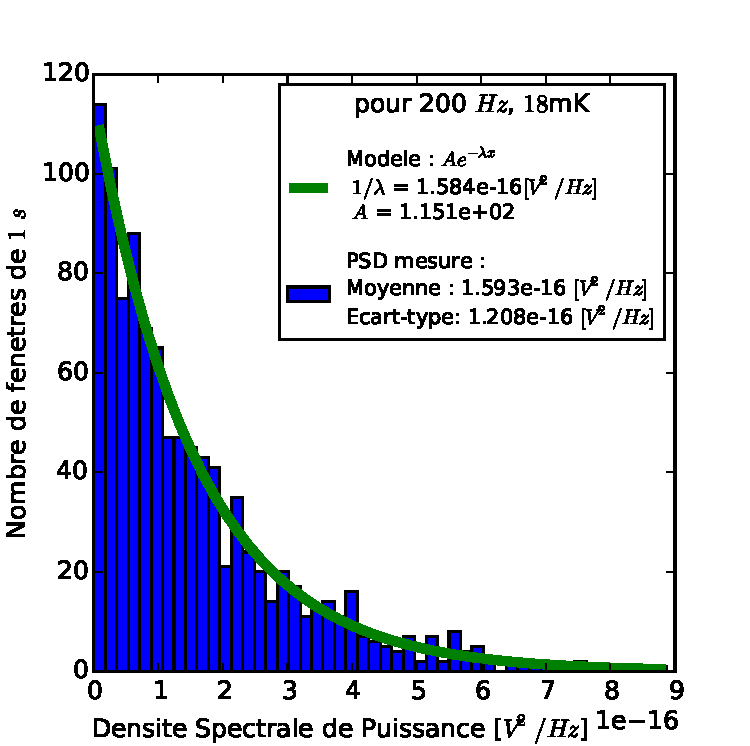
\includegraphics[width=0.6\textwidth]{Images/fit_exp_fin.pdf}
\end{center}
\caption{Histogramme de la densité spectrale de bruit à $200$ Hz ajustée par un modèle exponentiel.}
\label{noise-form}
\end{figure}

Dans un premier temps, on trace l'histogramme de la valeurs de la PSD mesurée pour différentes fréquences. Un tel histogramme est présenté pour une fréquence de $200$Hz sur la figure \ref{noise-form}. Quelque soit la fréquence sondée, la température du cryostat, ou l'électronique utilisée, on observe une forme de distribution analogue. On ajuste avec succès à ces histogrammes une distribution exponentielle. On peut appliquer au bruit une propriété de la loi exponentielle : la valeur moyenne $\mathcal{D}_i$ d'une mesure à la fréquence $i$ est égale à son écart-type $\sigma_{\mathcal{D}_i}$. En effet, les valeurs expérimentales de la moyenne et de l'écart-type sont proches du terme $1/\lambda$.
Ainsi, sur une mesure moyennée sur $N=120$ fenêtres de $1$ seconde, le Théorème Centrale Limite exprime l'écrat-type sur la mesure moyennée $\sigma_{\bar{\mathcal{D}}_i}$ tel que:
\begin{equation}
\label{sigma}
\sigma_{\bar{\mathcal{D}_i}} = \frac{\sigma_{\mathcal{D}_i}}{\sqrt{N}} = \frac{\bar{\mathcal{D}_i}}{\sqrt{120}}
\end{equation}

Cette information sur la PSD du bruit permet de construire rigoureusement une fonction de vraisemblance basée sur la fonction de $\chi^2$ relative au modèle de bruit avec les paramètres $\Theta$ et aux données expérimentales $\mathcal{D}$. Elle s'écrit :
\begin{equation}
\label{chi2}
\chi ^2 (\Theta|\mathcal{D}) = \sum^{N_{Temp}}_{j} \sum^{N_{bin}}_{i} \left[ \frac{\bar{\mathcal{D}_{ij}} - \mathcal{M}(f_{ij}; \Theta)}{\sigma_{\bar{\mathcal{D}_{ij}}}} \right]^2
\end{equation}
où on somme sur l'ensemble des fréquences $N_{bin}$ et sur l'ensemble des températures de mesure $N_{Temp}$. En effet, on ajuste simultanément le modèle sur plusieurs mesures de PSD effectuées pour des températures allant de $18$mK à $40$mK. On espère ainsi obtenir de meilleures contraintes sur les paramètres, d'abord parce qu'on analyse plus de points, mais surtout car le changement de température modifie des paramètres du système (en particulier la résistance du NTD $R(T_e)$) et permet de lever les problèmes de dégénérescence entre les différents paramètres libres.

Motivée par une approche bayésienne \cite{julien}, la fonction de vraisemblance s'exprime comme,
\begin{equation}
\label{likelihood}
\mathcal{L}(\Theta | \mathcal{D}) = \exp{\left(\frac{-\chi ^2 (\Theta|\mathcal{D})}{2}\right)}
\end{equation}


\subsubsection{Analyse par méthode de Monte Carlo avec Chaîne de Markov (MCMC)}


On recherche l'ensemble de paramètre $\Theta$ qui minimise la fonction de vraisemblance $\mathcal{L}(\Theta | \mathcal{D})$. On applique pour cela une analyse de Monte Carlo par Chaîne de Markov désignée comme méthode MCMC. Il s'agit d'une méthode reposant sur la marche aléatoire avec condition d'une (ou plus) chaine de Markov, un ensemble contenant les paramètres libres, dans l'espace de dimensions $N=7$ correspondant au nombre de paramètres libres. Il a été démontré \cite{julien} qu'avec une fonction de vraisemblance juste, la chaîne de Markov permet d'échantillonner cette fonction dans un voisinage de la solution optimale . Les avantages de la méthode MCMC sont qu'elle peut sonder une grande partie de l'espace des paramètres libres mais qu'elle converge rapidement vers le voisinage de solution optimale qu'il est alors possible d'explorer et d'analyser avec les histogrammes des positions des chaînes de Markov. La figure (\ref{triangle-mcmc}) présente de telles histogrammes pour l'électronique d'EDELWEISS.
\begin{figure}
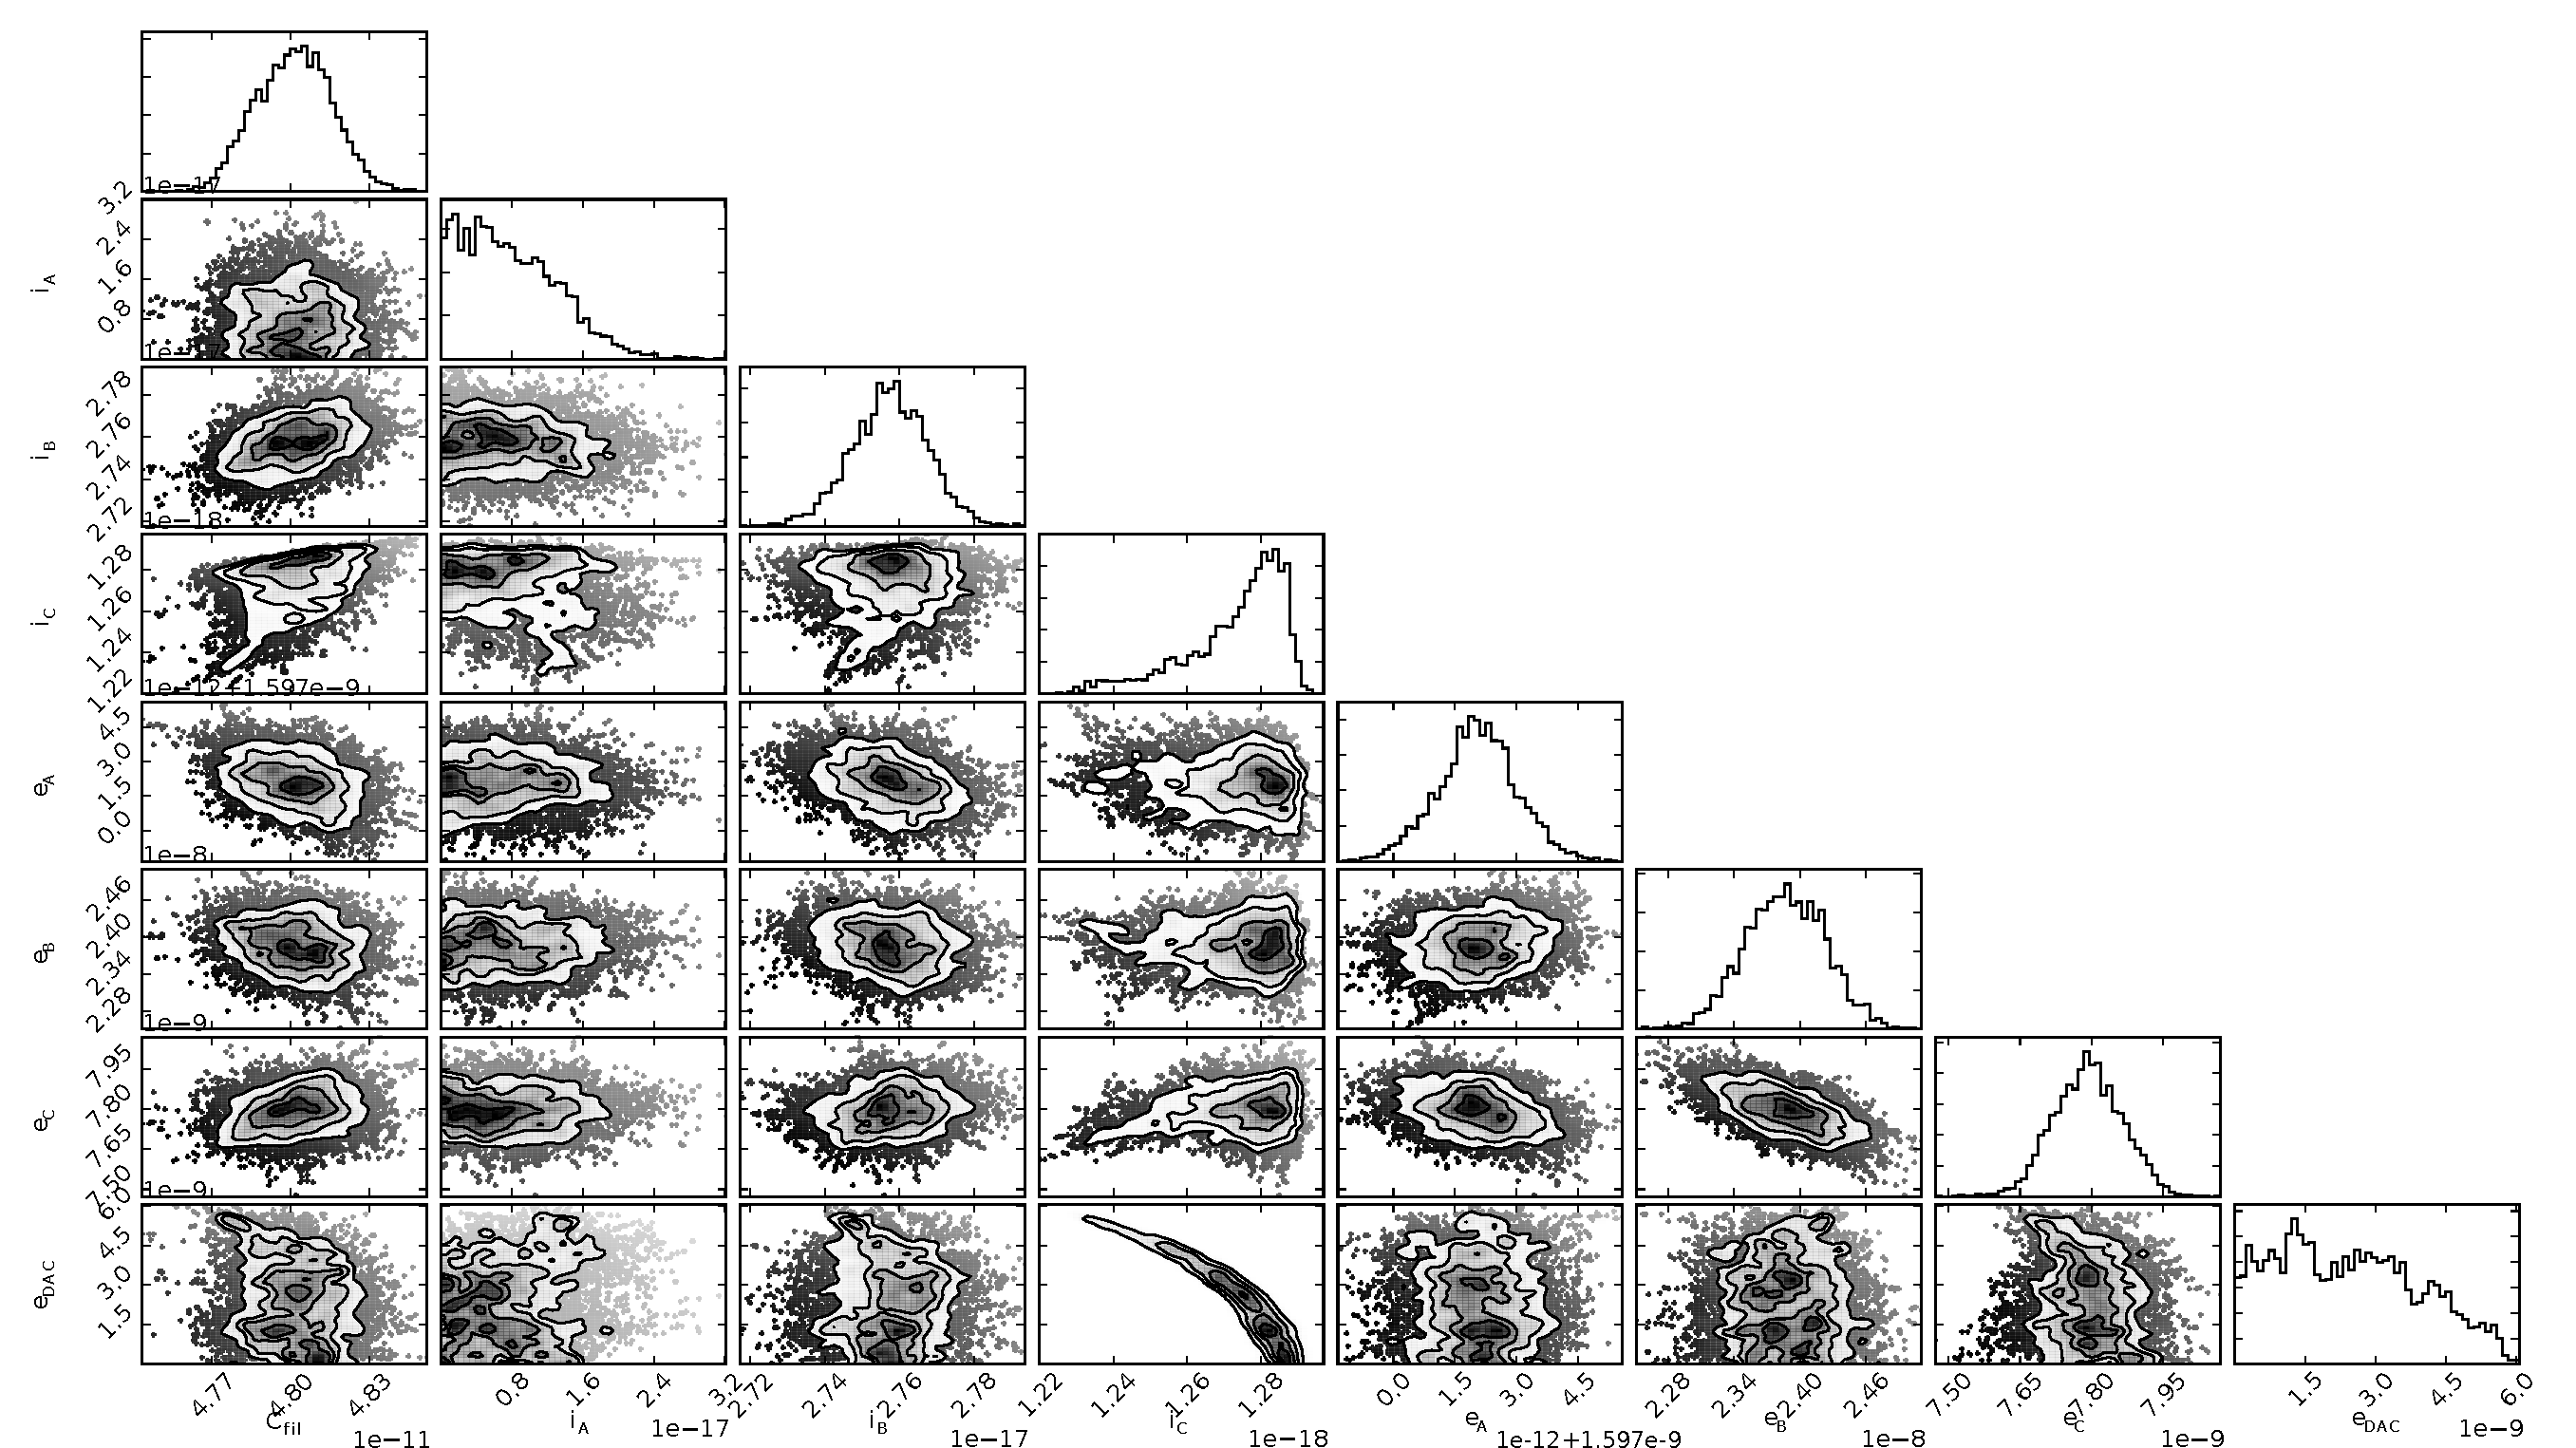
\includegraphics[width=\textwidth]{Images/triangle_fin.pdf}
\caption{Histogramme des positions des chaînes de Markov avec projections sur 2 dimensions, lors de l'analyse MCMC pour l'électronique EDELWEISS. Les paramètres libres présentés sont de haut en bas, et de gauche à droite : $C_{fil}, i_A, i_B, i_C, e_A, e_B, e_C, e_{DAC}$.}
\label{triangle-mcmc}
\end{figure}
On extrait de l'histogramme de positions la position moyenne comme estimation de l'ensemble de paramètres libres optimaux ainsi que les barres d'erreurs à 68\% sur cette estimation à partir des 16ème et 84ème quantiles des distributions. La forme des distributions nous renseigne également sur la qualité de contrainte imposée au paramètre considéré. En effet, une distribution étroite indique un paramètre bien contraint (paramètre $i_B$) avec des faibles barres d'erreurs contrairement à une distribution étalée qui présage de grandes barres d'erreurs (paramètre $i_A$). Deux paramètres dont la projection en 2 dimensions est allongée indique leur corrélation (paramètre $i_C$ et $e_{DAC}$). 

\begin{figure}[!ht]
\begin{center}
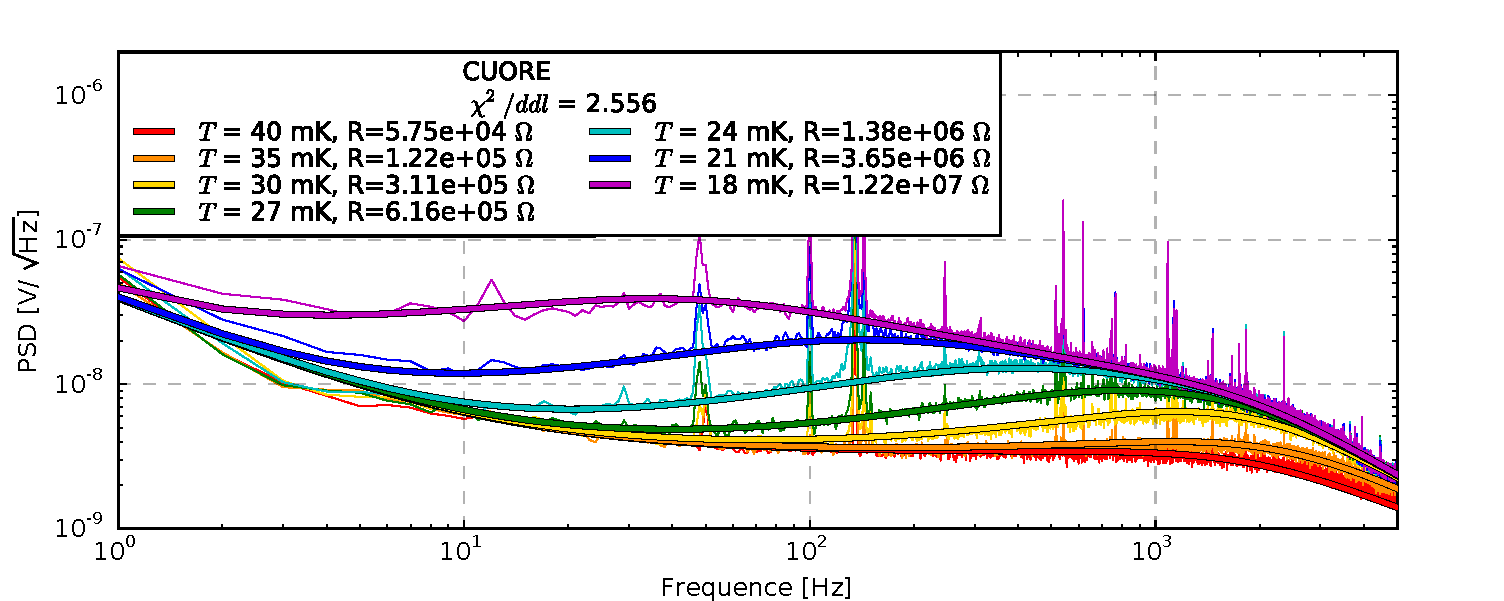
\includegraphics[width=\textwidth]{Images/cuore_fit_fin.pdf}
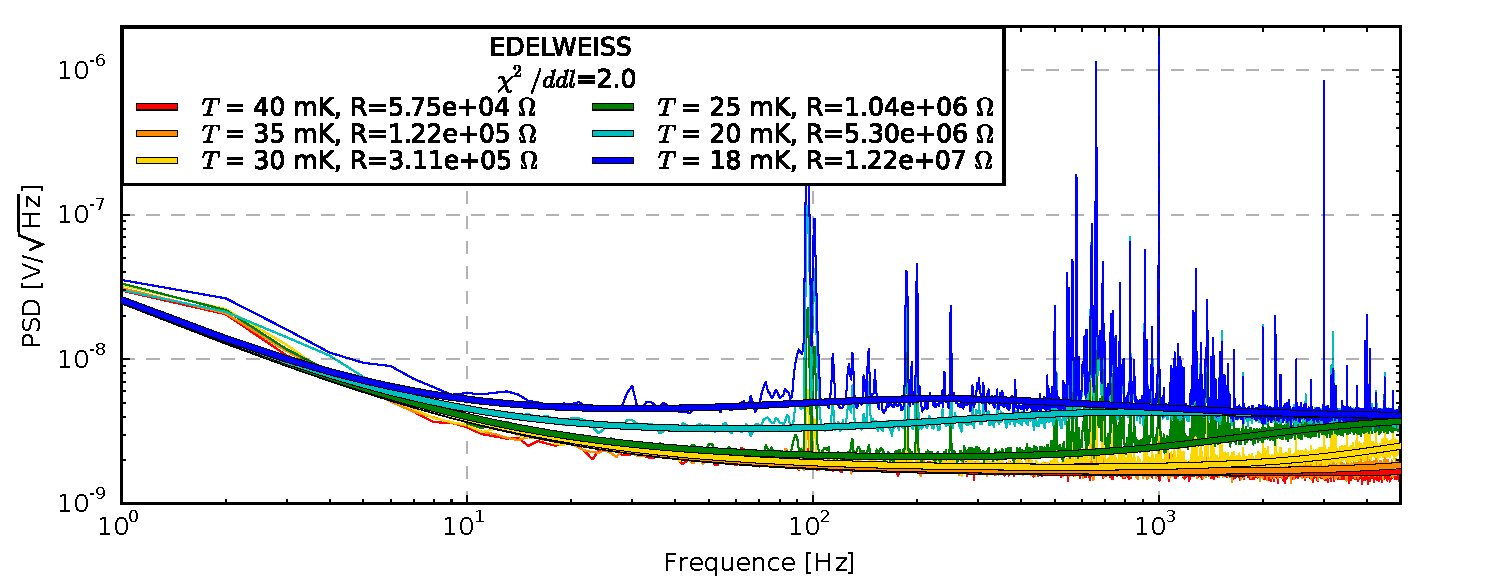
\includegraphics[width=\textwidth]{Images/edel_fit_fin.pdf}
\end{center}
\caption{Mesures moyennées (traits fins) et ajustement par analyse MCMC (traits épais) de densités spectrales de bruit pour différentes températures sur les deux électroniques : CUORE et EDELWEISS. Il est important de noter qu'il s'agit de mesures de bruit réalisées sans courant de polarisation. Pour chaque température de cryostat $T$ est précisée la valeur de la thermistance $R$. Le terme $\chi^2/ddl$ indique la valeur de la fonction $\chi^2$ divisée par le nombre de point (degrés de liberté) de l'ajustement. Pour une modélisation parfaite des données expérimentales : $\chi^2/ddl \rightarrow 1$}
\label{rainbow-plot}
\end{figure}

Après analyse MCMC, on obtient l'ajustement des données expérimentales relatives aux électroniques CUORE et EDELWEISS présenté dans la figure (\ref{rainbow-plot}). L'ajustement s'est effectué sur l'enveloppe des PSD, les pics parasites ont été ignorés pour l'analyse. Pour l'électronique CUORE, on observe une coupure au-delà de $2$kHz : cela provient d'un filtre passe-bas intégré à l'électronique. Il a été pris en compte et n'affecte donc pas la convergence du MCMC pour CUORE. On notera aussi l'apparition de deux paramètres libres supplémentaires. Le paramètre $f_B$ correspond à l'ordre du filtre passe-bas pour les mesures de CUORE. Le paramètre $e_{DAC}$ correspond au bruit d'une alimentation branchée en série avec la capacité de l'électronique EDELWEISS. L'ajout de ces paramètres supplémentaires permet d'apporter plus de souplesse au modèle pour qu'il s'adapte mieux aux données expérimentales, et ainsi de ne pas fausser la solution optimale.

\begin{align}
\label{result}
\begin{aligned}[c]
& \textrm{\textbf{CUORE}} \\
C_{fil} &= (2.94 \pm 0.01)\times 10^{-10}&[F] \\
i_A &= (1.9 \pm 0.03) \times 10^{-15}&[A/\sqrt{Hz}] \\
i_B &= (6.11 \pm 0.01) \times 10^{-16}&[A/Hz] \\
i_C &= (1.16 \pm 0.01) \times 10^{-17}&[A/Hz^{3/2}] \\
e_A &= (3.28 \pm 0.01) \times 10^{-9} &[V/\sqrt{Hz}] \\
e_B &= (3.03 \pm 0.04) \times 10^{-8}&[V] \\
e_C &= (1.08 \pm 0.02) \times 10^{-8} &[V \cdot \sqrt{Hz}] \\
f_B &= (2.70 \pm 0.01) & [u.a.]
\end{aligned}
\quad \vrule{} \quad
\begin{aligned}[c]
& \textrm{\textbf{EDELWEISS}} \\
C_{fil} &= (4.80 \pm 0.02)\times 10^{-11}&[F] \\
i_A &= (6.17 \pm 4.8) \times 10^{-18}&[A/\sqrt{Hz}] \\
i_B &= (2.76 \pm 0.01) \times 10^{-19}&[A/Hz] \\
i_C &= (1.28 \pm 0.02) \times 10^{-18}&[A/Hz^{3/2}] \\
e_A &= (1.60 \pm 0.00) \times 10^{-9} &[V/\sqrt{Hz}] \\
e_B &= (2.39 \pm 0.04) \times 10^{-8}&[V] \\
e_C &= (7.81 \pm 0.07) \times 10^{-9} &[V \cdot \sqrt{Hz}] \\
e_{DAC} &= (2.02 \pm 1.9) \times 10^{-9}&[V/\sqrt{Hz}] 
\end{aligned}
\end{align}

On vérifie bien que l'ajustement est excellent sur l'ensemble des fréquences, avec pourtant une certaine réserve pour les basses fréquences de l'électronique CUORE. En effet, la fonction de $\chi^2$ pondérée par le nombre de degrés de libertés $ddl$ est égale à $2.556$ pour CUORE et $2.0$ pour EDELWEISS, ce qui se rapproche de la valeur $1$ correspondante à une modélisation parfaite. Les solutions optimales, indiquées en (\ref{result}), pour les électroniques permettent de bien simuler le bruits des électroniques à partir du modèle proposé (\ref{i-ampli}, \ref{e-ampli}). On observe des comportements différents suivant la température du cryostat.  En notant, grâce à l'équation (\ref{ode-mat}) et au diagramme \ref{block-diagram}, que la contribution du bruit en courant $i_{bruit}$ augmente avec l'impédance complexe $Z_{eq}$, on peut expliquer que les niveaux de PSD sont plus élevés à basse température. En effet, la résistance NTD $R(T_e)$ croît très fortement quand la température du cryostat décroît, ainsi l'impédance complexe $Z_{eq}$ s'en retrouve également augmentée.

Le comportement à basse fréquence des deux électroniques est très similaire : on observe une forte remontée à basse fréquence associée aux paramètres $e_{B,C}$. À plus haute fréquence, on note que l'électronique de CUORE est beaucoup plus sensible à la température que EDELWEISS. Pour toute les températures, le niveau de bruit de l'électronique CUORE est supérieur à celui de EDELWEISS. On a simplement un facteur 2 à $40$mK tandis qu'on a presque un ordre de grandeur de différence à $18$mK. Les résultats \ref{result} montrent une différence de deux ordre de grandeur entre le bruit en courant $i_A$ de CUORE et celui de EDELWEISS. Celui-ci se couple à l'impédance complexe $Z_{eq}$ et explique le niveau de bruit mesuré.

\begin{figure}[!ht]
\begin{minipage}{0.49\textwidth}
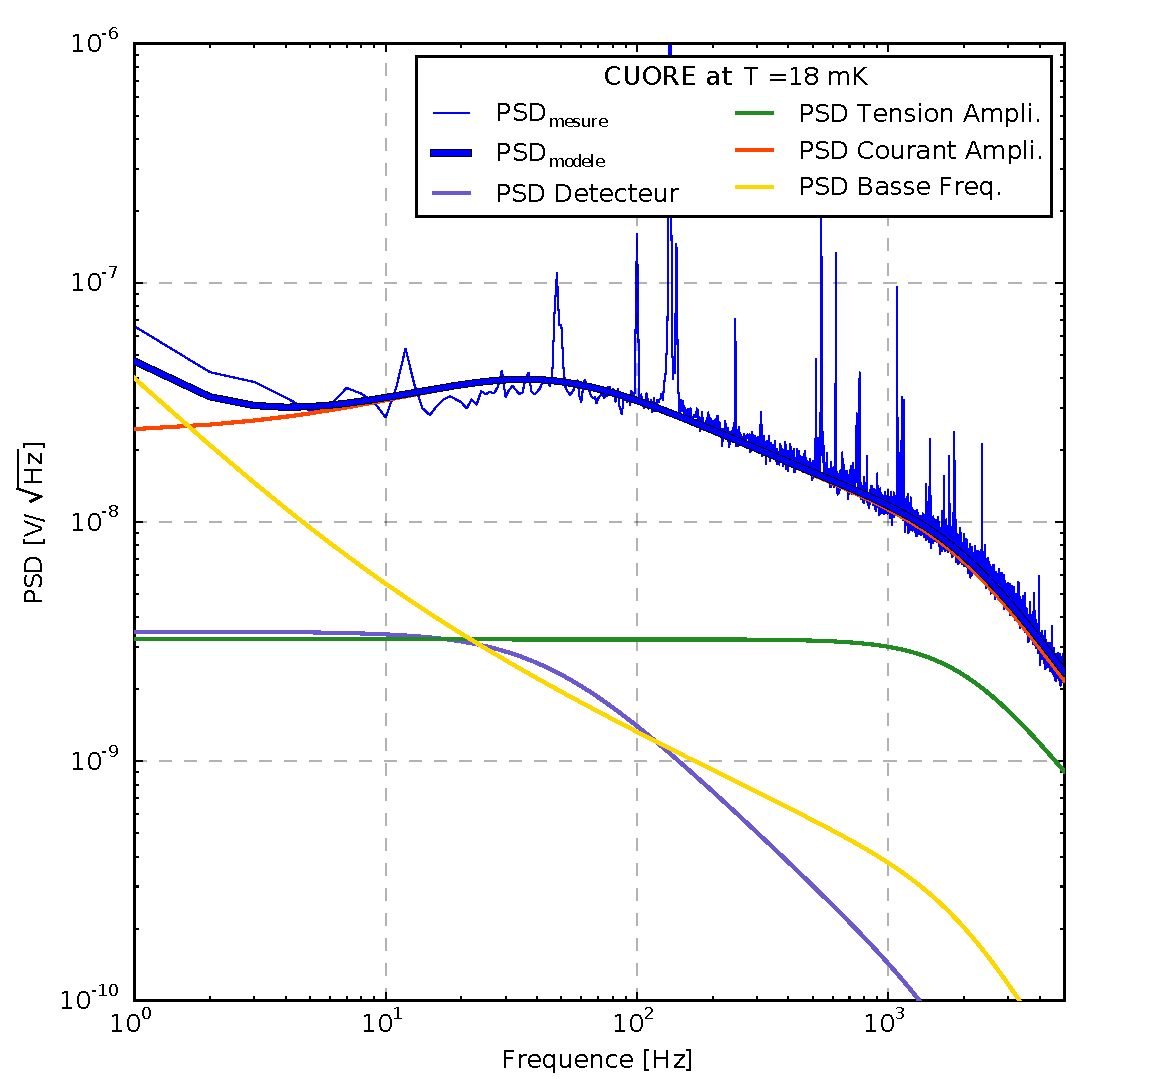
\includegraphics[width=\textwidth]{Images/cuore_18.pdf}
\end{minipage}
\hfill
\begin{minipage}{0.49\textwidth}
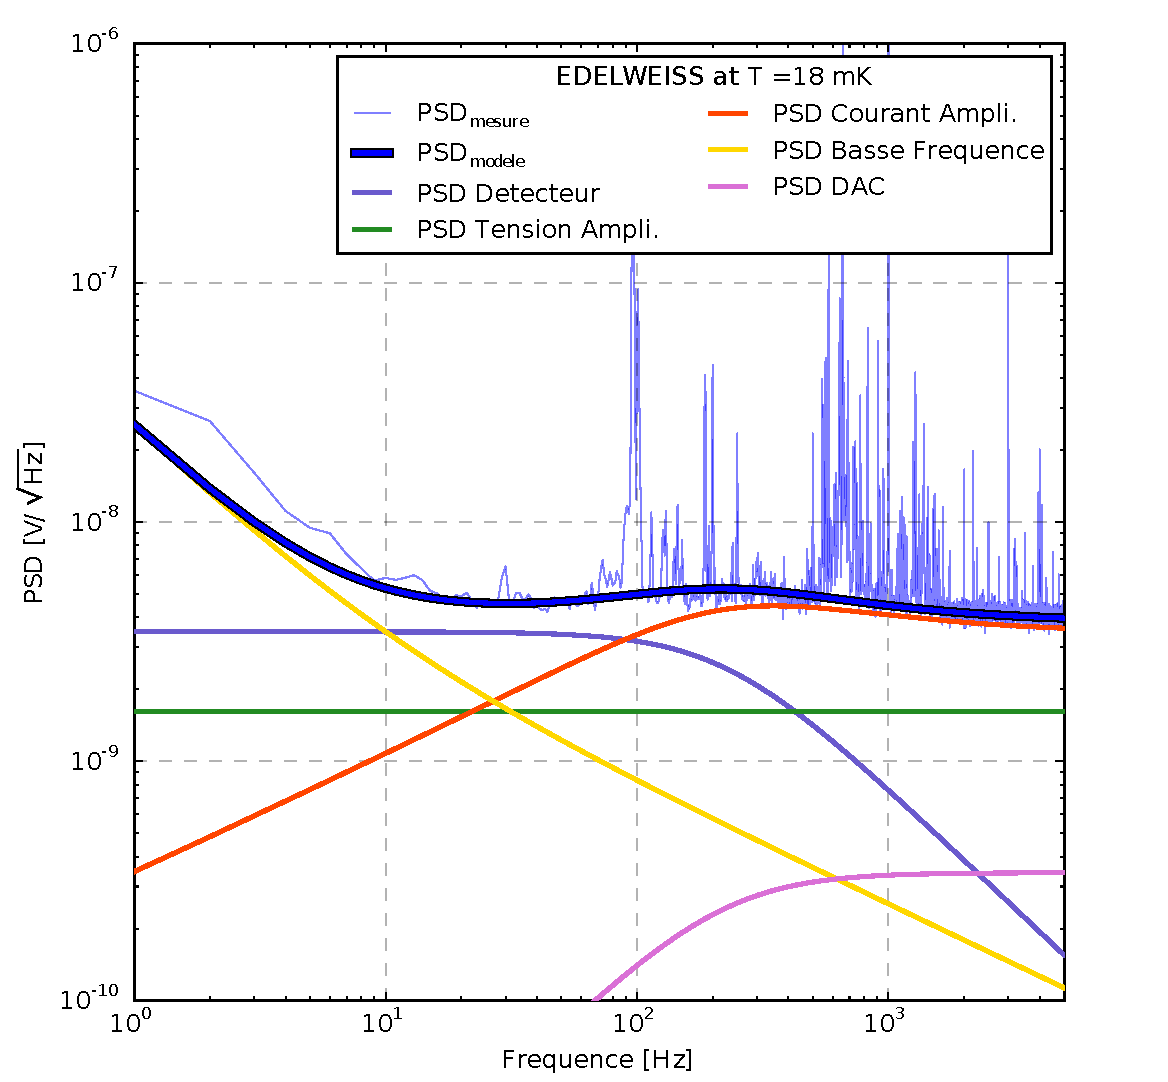
\includegraphics[width=\textwidth]{Images/edel_18.pdf}
\end{minipage}
\caption{Mesure expérimentale et modèle d'une densité spectrale de bruit à $18$ mK pour les électroniques CUORE (à gauche) et EDELWEISS (à droite) avec visualisation des contributions des différentes sources de bruits.}
\label{noise-sources}
\end{figure}

Il apparaît donc que l'électronique la moins bruyante est celle d'EDELWEISS. C'est donc avec cette électronique qu'il est convenu d'optimiser la résolution des détecteurs. Néanmoins, l'électronique EDELWEISS nécessite certaines modifications afin d'être utilisée avec une polarisation non nulle (remplacer la capacité par une résistance de charge). Cela étant à l'état de projet, on ne peut utiliser que l'électronique CUORE pour les mesures avec polarisation pour caractériser le détecteur RED10. Comme elle a également été caractérisé, cela ne pose pas de problèmes particuliers.

En utilisant la solution optimale trouvé avec l'analyse MCMC, il est possible de visualiser les contributions des différentes sources de bruits à la PSD de bruit totale, un exemple à $18$mK est présenté en figure \ref{noise-sources} pour les électroniques de CUORE et EDELWEISS. On constate bien que le bruit en courant de CUORE est très élevé et prédomine presque toute la gamme en fréquence. La fréquence de coupure du bruit Johnson, différentes pour les deux électroniques, illustre bien l'influence de la capacité du câblage. En effet, on a $f_{coupure} = 2\pi/(R_{NTD} C_{fil})$ en considérant $R_L\gg R_{NTD}$. On retrouve bien une fréquence de coupure plus élevée dans le cas de EDELWEISS qui possède une capacité de câblage plus faible (voir \ref{result}). Il est aussi possible d'étudier la prédominance des sources de bruits en fonction de la fréquence. Pour l'électronique d'EDELWEISS :
\begin{itemize}
\item en dessous de $10$Hz, le bruit est dominé par la contributions basse fréquence du bruit en tension $e_{B,C}$.
\item de $10$Hz à $100$Hz, le bruit totale vient se reposer sur le bruit intrinsèque au détecteur (bruit TFN et bruit Johnson du NTD). C'est exactement ce qui est recherché : on cherche à être limité par ces bruits thermiques détecteurs qui fixe la limite ultime atteignable.
\item au-dessus de $100$Hz, le bruit en courant de l'électronique d'amplification caractérisé par les coefficients $i_{A,B,C}$ devient prédominante.
\end{itemize} 

\begin{figure}[!ht]
\begin{minipage}{0.49\textwidth}
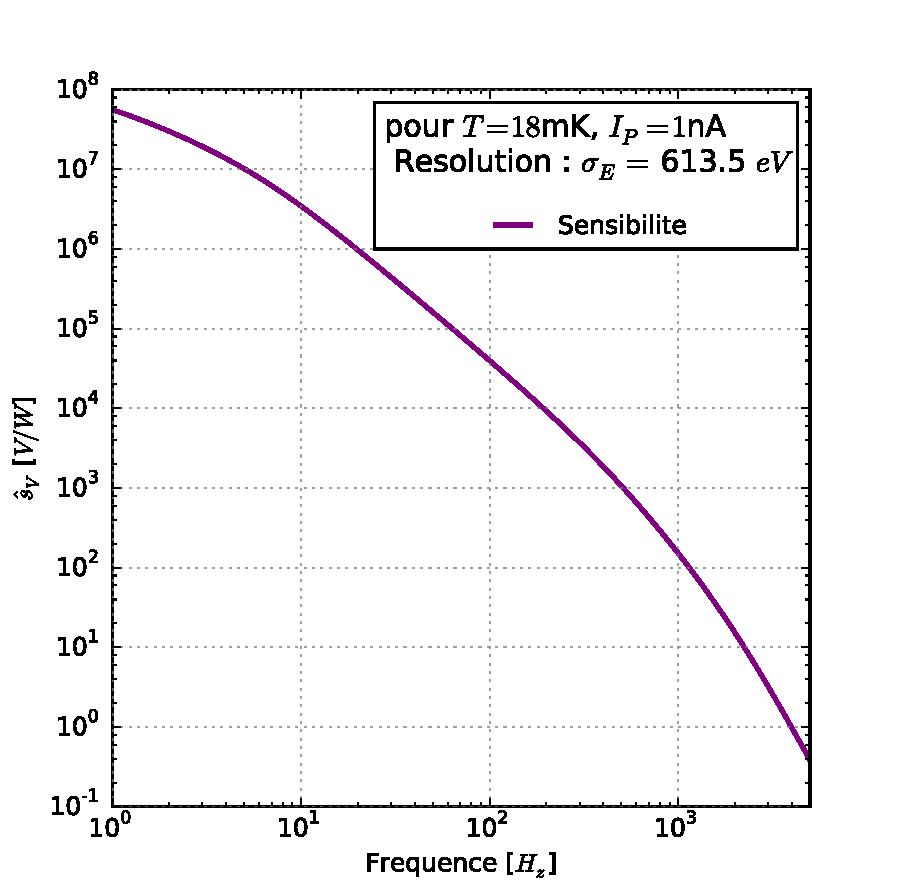
\includegraphics[width=\textwidth]{Images/sv_fin.pdf}
\end{minipage}
\hfill
\begin{minipage}{0.49\textwidth}
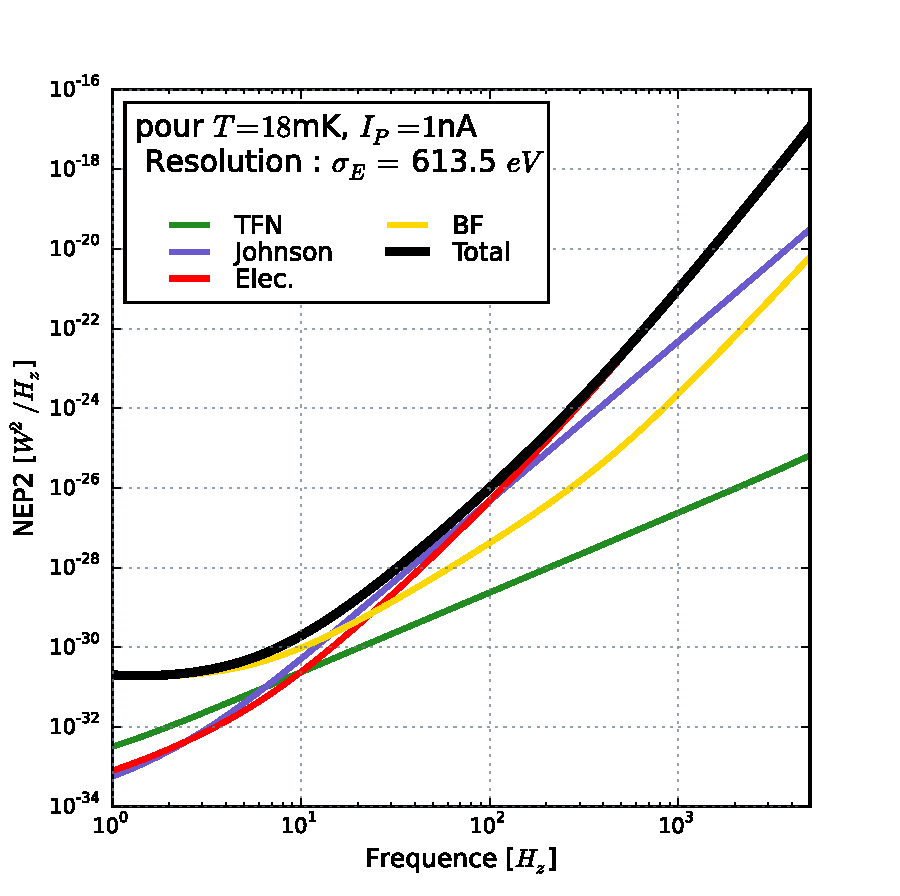
\includegraphics[width=\textwidth]{Images/nep_fin.pdf}
\end{minipage}
\caption{Simulation de la sensibilité (à gauche) et de la NEP (à droite) avec contributions des différentes sources de bruit pour l'électronique EDELWEISS à une température cryostat de $T=18$mK et un courant de polarisation de $1$nA.}
\label{nep-fig}
\end{figure}

\subsubsection{Tracé de la NEP et calcul de la résolution}
\label{nep-res}

Maintenant que l'on a contraint tous les paramètres du modèle de bruit, il est possible de finaliser le calcul de la résolution \ref{resolution} avec le calcul de la NEP \ref{nep}. La figure \ref{nep-fig} présente des graphes de sensibilité et de NEP du détecteur avec l'électronique EDELWEISS à $18$mK pour un courant de polarisation de $1$nA. La sensibilité est conforme avec la fonction de transfert d'un système thermique : il s'agit bien d'un passe-bas. Combiner selon la formule (\ref{nep}) cette sensibilité avec la PSD de bruit totale caractérisée précédemment permet d'obtenir une simulation de la NEP qui présente ses plus faibles valeurs entre $1$Hz et $100$Hz. 

%\begin{figure}[!ht]
%\begin{center}
%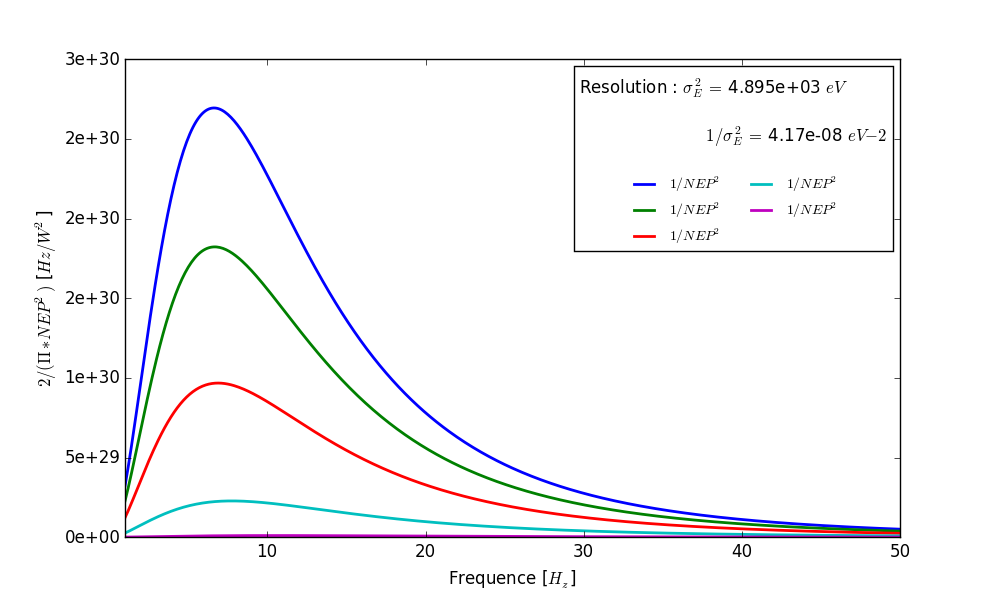
\includegraphics[width=0.7\textwidth]{Images/inte.png}
%\end{center}
%\caption{Simulation de la fonction $\frac{2}{\pi \times NEP^2(\omega)}$ qui apparaît comme intégrande dans la formule de la résolution (\ref{resolution}).}
%\label{inte}
%\end{figure}

Il est maintenant possible d'accéder à la résolution des cette configuration d'expérience avec la formule (\ref{resolution}). On calcule ici une résolution de $613.15$eV pour EDELWEISS, et une résolution de $1061.7$eV pour CUORE, avec une température de $18$mK et un courant de polarisation de $1$nA. On obtient bien une valeur inférieure avec l'électronique EDELWEISS, ce qui confirme davantage le choix de cette électronique pour l'optimisation de la résolution.

La formule du calcul de la résolution (\ref{resolution}) indique que les valeurs de NEP les plus basses contribuent le plus à la résolution. Même si intégrer sur une plus grande gamme de fréquence permet d'obtenir une résolution plus faible, le gain devient négligeable à mesure que la valeur de la NEP augmente.
On note que la NEP prend ses valeurs minimales au voisinage de $10$Hz : la majorité de l'information de la mesure est contenue dans une plage en fréquence allant de $0$Hz à environ $50$Hz. Le gain sur la résolution en intégrant au-delà de $50$Hz est infime. On cerne alors la plage de fréquence d'intérêt pour l'étude du signal. En observant les contributions des différentes sources de bruits à la NEP à la figure \ref{nep-fig}, on s'aperçoit que c'est le bruit basse fréquence qui domine dans cette plage de fréquence d'intérêt, suivi par le bruit Johnson de la résistance NTD. On comprend que pour diminuer davantage la résolution de ces détecteurs, il faut travailler à augmenter la sensibilité du système à un évènement ou réduire le bruit basse fréquence. Une partie de l'équipe Manoir travaille déjà à comprendre ce bruit basse fréquence.

\subsection{Caractérisation thermique du détecteur RED10}

Le détecteur RED10 n'est entré en possession du groupe Manoir que très récemment. Son design est identique à celui de RED1. La différence avec ce dernier repose dans le type de colle utilisée (colle de l'expérience CRESST) et les dimensions du NTD utilisé. Certains paramètres thermiques sont alors modifiés par rapport à RED1. Il est ainsi nécessaire de caractériser ces paramètres thermiques pour nouveau détecteur. On pourra ainsi étudier sa réponse à un évènement comme cela été fait avec RED1 dans les parties précédentes.

\subsubsection{Caractéristique courant-tension et forme du signal}

La caractérisation des paramètres thermiques utilise le modèle électro-thermique qui a été construit précédemment. On va vouloir ajuster les paramètres non contraints aux données expérimentales avec une analyse MCMC comme pour la caractérisation de l'électronique. Cette fois-ci, l'ensemble des paramètres libres est :
\begin{equation}
\Theta = (R_0, T_0, g_{ep}, g_k, g_{glue}, \epsilon, \tau_P)
\label{theta-red10}
\end{equation}
En effet, la nouvelle colle utilisée possède une conductivité $g_{glue}$ différente. La nouvelle géométrie du NTD (et également son dopage en neutron légèrement différent) va entraîner une modification de la résistance $R_0$ et température caractéristique $T_0$ présent dans l'équation (\ref{ntd}). Le changement de dimension impacte également le couplage électron-phonon $g_{ep}$ et le coefficient de conduction Kapitza $g_k$. A priori, les capacités thermiques volumiques de l'absorbeur et du NTD restent inchangées, ce qui permet de recalculer les nouvelles capacités thermiques à partir des dimensions connues du NTD. Il aurait été possible d'inclure celles-ci dans les paramètres libres mais le choix de les fixer a été favorisé afin d'éviter les problèmes de dégénérescence et ainsi mieux contraindre les paramètres.

Une étude préliminaire de la forme du signal (présenté à droite de la figure \ref{v2i-red10}) de RED10 a révélé que la décroissance de l'impulsion possède deux constantes de temps caractéristiques. Ce type de signal n'a jamais été observé sur les mesures de signal réalisée avec RED1 : il n'y a qu'un seul temps caractéristique de décroissance expliqué par la fuite thermique vers le cryostat depuis la bain d'électron avec un dépôt d'énergie de recul dans l'absorbeur. La présence d'un deuxième temps caractéristique pour RED10 ne peut s'expliquer que par la présence de phonons athermiques comme introduit dans la section \ref{omega}. Il s'agit de phonons ne se relaxant pas de suite dans l'absorbeur, mais passant dans le senseur NTD avant de s'y relaxer. Ils créent ainsi une élevation de température directement au sein du NTD. Le terme de source $\bm{F}$ de l'équation (\ref{ode-mat}) se réécrit alors :
\begin{equation}
\bm{F}(t-t_0) = 
\left( \begin{array}{c}
(1-\epsilon)E/C_a \\
0 \\
\epsilon E/C_e \\
0
\end{array} \right) \delta (t-t0)
\end{equation}
avec $\epsilon$ la fraction d'énergie de recul convertie en phonons athermiques. Les constantes de normalisation de la solution temporelle générale (\ref{eigein-solc-expr}) dépendent du terme de source $\bm{F}$ d'après (\ref{normal}) et diffèrent alors du cas de RED1 sans phonons athermiques. Cela a pour effet de mieux exprimer une nouvelle exponentielle, et donc un nouveau temps caractéristique, contenue dans la solution générale. Cette observation de deux temps caractéristiques pour le signal motive l'ajout de la fraction de phonons athermiques $\epsilon$ et de leur temps caractéristique de relaxation $\tau_P$ au paramètres libres du modèle.

On mesure sur RED10 les caractéristiques courant-tension et la forme du signal à un évènement de la radioactivité naturelle à courant de polarisation fixe $I_P=4$nA pour différentes températures allant de $18$mK à $30$mK. On étudie ainsi le comportment de RED10 dans l'état stationnaire (section \ref{steady-section}) et en régime temporel (section \ref{temporal}).
On effectue l'analyse par fonction de vraisemblance avec la méthode MCMC comme dans la section \ref{caract}. Les données expérimentales avec les modèles ajustés sont présentés sur la figure (\ref{v2i-red10}).

\begin{figure}[!ht]
\begin{minipage}{0.49\textwidth}
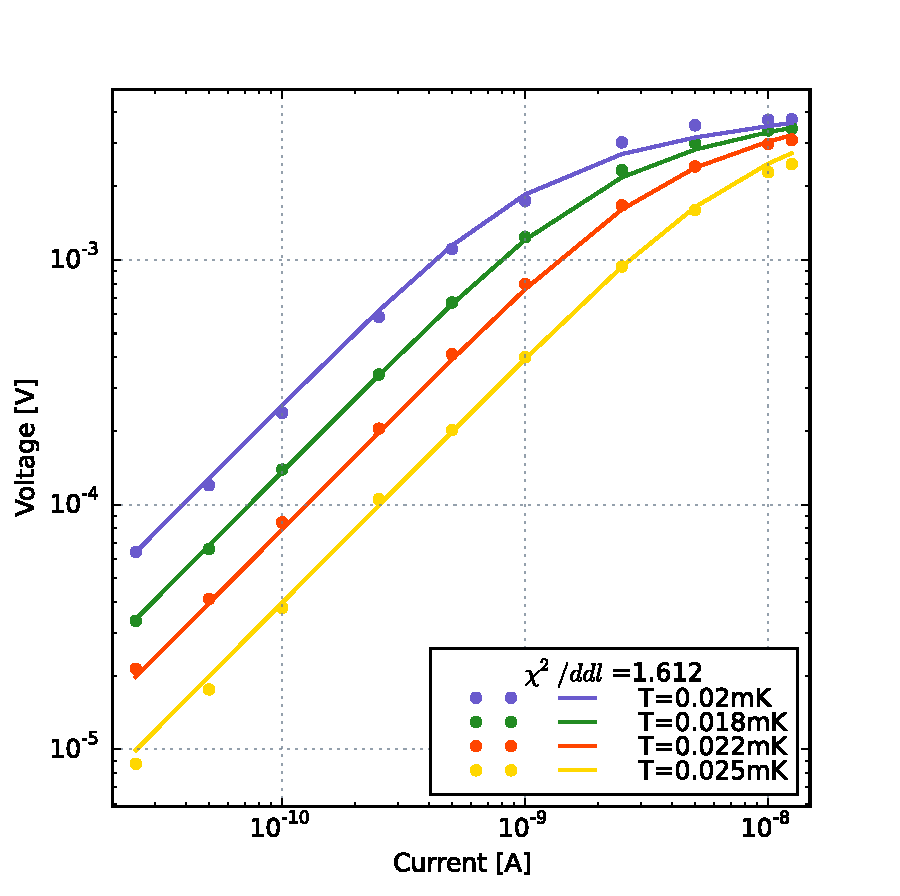
\includegraphics[width=\textwidth]{Images/v2i_red10.pdf}
\end{minipage}
\hfill
\begin{minipage}{0.49\textwidth}
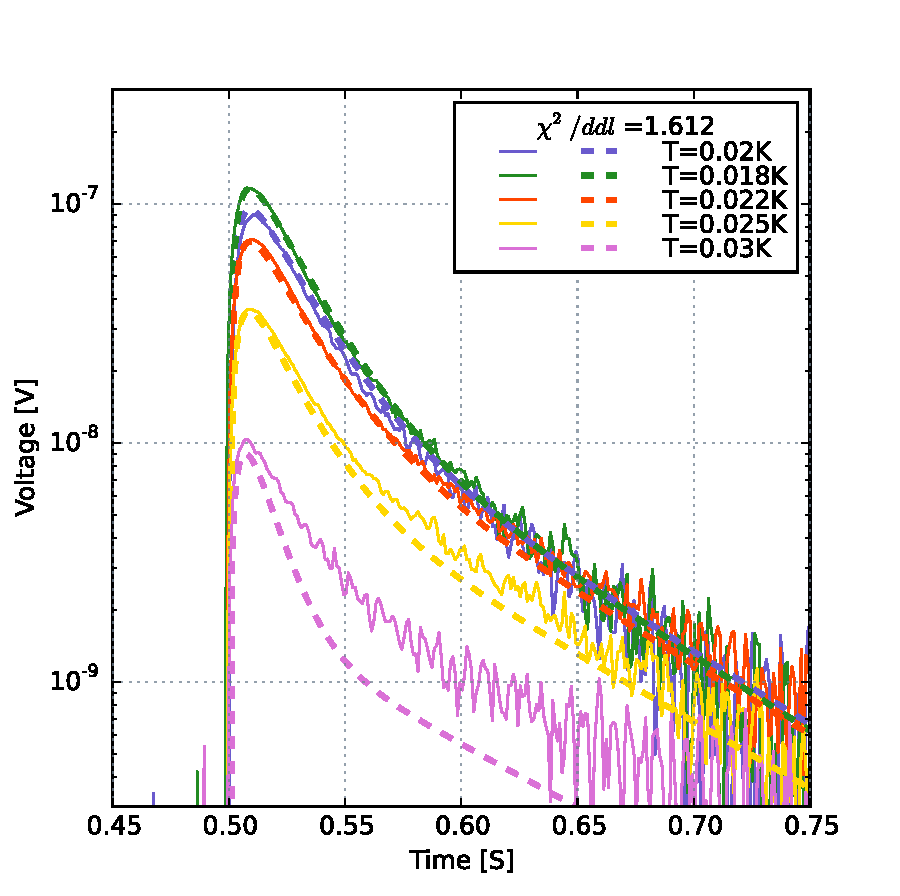
\includegraphics[width=\textwidth]{Images/pulse_red10.pdf}
\end{minipage}
\caption{Mesure expérimentale et ajustement par le modèle de la caractéristique courant-tension (à gauche) et  d'un signal créé par un évènement de radioactivité ambiante (à droite) pour le détecteur RED10.}
\label{v2i-red10}
\end{figure}

L'ajustement semble bon pour les deux types de mesure avec $\chi^2/ddl=1.612$. On observe néanmoins une difficulté de l'ajustement du pulse pour une température de $30$mK. La caractéristique courant-tension permet de contraindre les paramètres libres intervenant dans les équations de l'état stationnaire : $R_0, T_0, g_{ep}, g_k$. L'analyse de ces équations (\ref{steady}) nous donne que la partie linéaire de la caractéristique contraint surtout la valeur de résistance du NTD, et donc $R_0, T_0$. Le palier en tension à plus haut courant de polarisation provient d'un effet Joule excessif qui n'est alors plus compensé par la fuite thermique vers le cryostat. Le NTD augmente alors en température, perdant en résistance électrique avec un courant de polarisation constant, ce qui produit l'apparition du palier de tension. Son ajustement contraint ainsi les valeurs des conductivités $g_k$ et de couplage électron-phonon $g_{ep}$.

Pour ce qui est de la forme du signal, le modèle fait en effet apparaître deux pentes et donc deux temps caractéristiques. L'ajustement de ces deux pentes de décroissance contraint la fraction de phonon athermique $\epsilon$, et de manière plus générale, tous les paramètres intervenant dans le calcul des constantes de normalisation de la base propre des solutions (\ref{eigen-soluc}).
La montée en tension permet de contraindre le temps de relaxation des phonons $\tau_P$. En effet, pour une relaxation immédiate des phonons, le temps de montée serait infiniment grand (modulo la fréquence de coupure $(RC_{fil})^{-1]}$).

La méthode MCMC donne alors les contraintes suivantes pour RED10:

\begin{align}
R_0 &= (11.6 \pm 0.4)&[\Omega] \\
T_0 &= (2.72 \pm 0.01) &[K] \\
g_{ep} &= (21.1 \pm 4.4) &[W/K^6/cm^3] \\
g_k &= (2.77 \pm 0.1) \times 10^{-4}&[W/K^4/mm^2] \\
g_{glue} &= (7.46 \pm 1.67) \times 10^{-4} &[W/K^{n_g}/mm^2] \\
\epsilon &= (0.202 \pm 0.001)  & [fraction]\\
\tau_P &= (4.03 \pm 0.03) \times 10^{-3} &[s]
\end{align}

Ces valeurs de paramètres thermiques sont du même ordre de grandeur que celles correspondantes à RED1. Il est important de mettre en évidence la forte portion de phonons athermiques d'environ $20\%$ qui est à comparer à leur absence complète avec le détecteur RED1. Il s'agit d'une observation encore inédite pour ce type de détecteur. Leur présence élevée se traduit par une accélération du signal en tension et donc une augmentation de la gamme de fréquence d'intérêt du signal introduit dans la section \ref{nep-res}. De plus, les phonons athermiques ne sont pas affectés par la capacité de l'absorbeur, et transmettent directement l'ensemble de leur énergie au NTD. La compréhension et l'augmentation du taux de phonons athermiques permettrai ainsi d'abaisser la résolution du détecteur. On a ainsi découvert une nouvelle voie d'optimisation des détecteurs encore non considérée au sein de la collaboration EDELWEISS.

\subsubsection{Bruit et résolution de RED10}

Comme RED10 est complètement caractérisé du point de vue thermique, et que l'électronique CUORE utilisée pour les mesures l'est également, nous sommes en mesure de simuler le spectre de bruit lié à RED10 que l'on compare à la mesure expérimentale. La figure (\ref{noise-red10}) présente la modélisation et la mesure expérimentale de la PSD du bruit de RED10 à courant de polarisation de $4$nA pour une température de $22$mK. On notera qu'un filtre de Bessel est appliqué à la mesure, et au modèle, ce qui explique la coupure apparaissant à partir de $2$kHz.

\begin{figure}[!ht]
\begin{center}
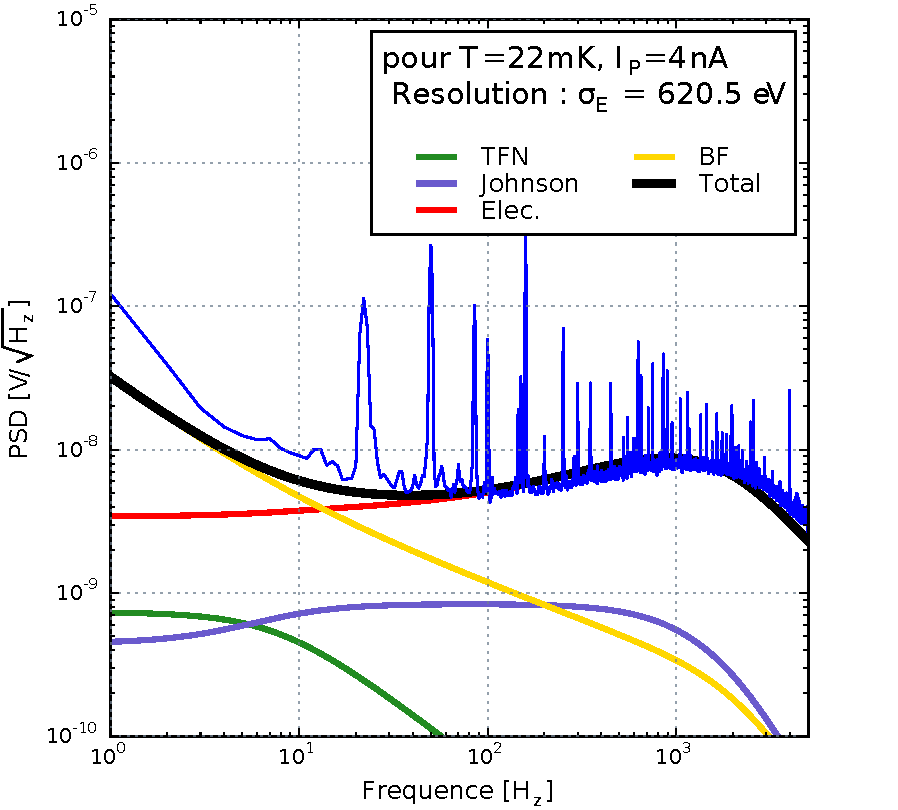
\includegraphics[width=0.55\textwidth]{Images/modexp.pdf}
\end{center}
\caption{Mesure expérimentale d'une densité spectrale à $22$ mK avec RED10 comparée à une simulation du modèle construit.}
\label{noise-red10}
\end{figure}

Le modèle et la mesure décrivent des évolutions très similaires. On retrouve effectivement la présence d'un bruit basse fréquence élevé qui domine jusqu'à $15$Hz. C'est ensuite le bruit en courant qui prédomine sur le reste de la gamme de fréquence. On notera qu'on effectue ici une mesure de bruit avec courant de polarisation, il serait donc incorrect de vouloir comparer le bruit en courant présenté de RED10 avec les bruits en courant de RED1 obtenus sans courant de polarisation. On observe toutefois un léger glissement du modèle par rapport aux données expérimentales vers les basses fréquences. Cela peut être expliqué par la sous-estimation du bruit basse fréquence déjà observé pour l'électronique de CUORE à la figure (\ref{rainbow-plot}). L'excès de bruit basse fréquence provient également du taux important d'évènements muons durant les mesures : malgré les coupures effectuées en analyse, on récupère toujours une partie de la décroissance des signaux, ce qui participe à amplifier les basses fréquences du spectre mesuré.

La mesure de résolution expérimentale s'effectue à partir des PSD de bruit et de la mesure d'un signal. En effet, renormaliser l'amplitude du signal et lui appliquer une méthode de Welch permet d'estimer la sensibilité en signal du détecteur RED10. La renormalisation nécessite également de connaître la conversion entre l'énergie déposée dans l'absorbeur par un évènement et l'amplitude du signal mesurée. Cette calibration s'effectue à l'aide de l'interaction des muons cosmiques avec l'absorbeur. L'énergie qu'ils déposent dans l'absorbeur est égale à $18$MeV. La mesure de l'amplitude en tension d'un signal muon permet donc d'en déduire le facteur de conversion nécessaire à la renormalisation d'un signal. L'application de l'analogue discrète de la formule (\ref{resolution}) à un spectre de bruit et la sensibilité calculée précédemment  permet l'évaluation d'une résolution expérimentale. 

\begin{figure}[!ht]
\begin{center}
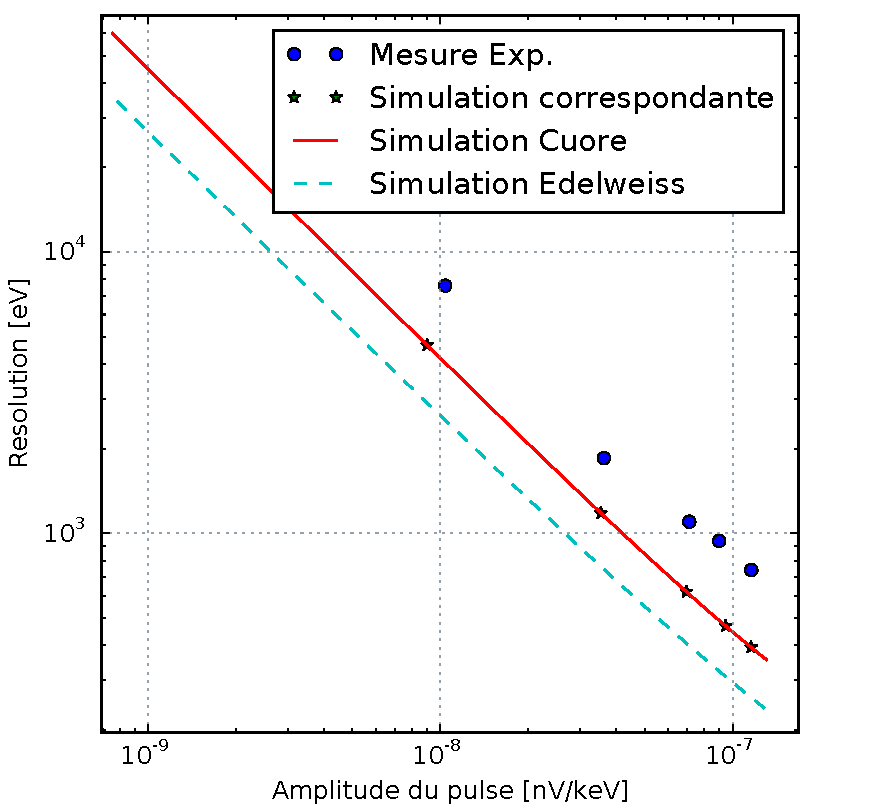
\includegraphics[width=0.55\textwidth]{Images/resamp_fin_fin.pdf}
\end{center}
\caption{Caractéristique Résolution-Amplitude de signal pour le détecteur RED10 pour un courant de polarisation de $4$nA avec des températures allant de $18$mK à $30$mK.}
\label{amp-res-red10}
\end{figure}

On présente sur la figure (\ref{amp-res-red10}) les résolutions en fonction de l'amplitude du signal pour différentes températures à courant de polarisation fixé. Les résolutions expérimentales sont plus élevées que les résolutions simulées. Cela s'explique par la déviation entre modèle et mesure de bruit observée en figure (\ref{noise-red10}): le bruit basse fréquence modélisé est plus bas qu'en réalité, d'où la prédiction de résolutions plus basses. L'amplitude des pulses permet d'estimer la sensibilité de RED10 au signal. Hormis la mesure à $30$mK dont le signal était déjà mal modélisé, les valeurs d'amplitude simulées et réelles sont quasiment identiques. De plus, comme les deux ensembles de points présentent une évolution de la résolution en fonction de l'amplitude très similaire, on en déduit que le modèle est en bonne adéquation avec la réalité expérimentale. Une étude de la différence sur le bruit est encore nécessaire pour obtenir une adéquation complète de modèle et de l'expérience.

On notera qu'on a effectué les mesures avec l'électronique de CUORE. La simulation de la caractéristique résolution-amplitude est tracée pour les deux électroniques CUORE et EDELWEISS. On note que cette dernière permet de gagner quasiment un facteur 2 sur la valeur de la résolution (l'amplitude reste inchangée). Ce qui est cohérent avec le faible niveau de bruit de EDELWEISS par rapport à celui de CUORE.

\subsection{Optimisation du détecteur RED10 et perspectives}

Un modèle électro-thermique a été construit et testé avec RED10. Même si quelques paramètres méritent d'être davantage affinés pour avoir un meilleur ajustement, nous pouvons réaliser une optimisation préliminaire du détecteur RED10. On présente à la figure \ref{optim} une simulation de la résolution de RED10 en fonction de courant de polarisation parcourant son NTD pour différentes température de cryostat. La simulation est effectuée avec l'électronique EDELWEISS qui possède le niveau de bruit le plus faible, et on abaisse la température de la résistance de charge à la température de la chambre de mélange pour réduire son bruit Johnson (ce qui sera réalisé dans ces prochains mois).

On observe qu'il existe un optimum de courant correspondant à chaque température permettant de minimiser la résolution. En effet, si on polarise trop la thermistance NTD, la chaleur produite par effet de Joule ne peut plus être évacuée efficacement par la fuite thermique. La température du NTD devient haute et donc sa valeur baisse, ce qui affecte la sensibilité du système. Ce même effet est observé lors du tracé de la caractéristique courant-tension en figure \ref{v2i-red10}. À trop faible courant, le senseur NTD n'est plus assez polarisé pour convertir efficacement le signal chaleur en un signal tension : la sensibilité chute également. Quelque soit le courant de polarisation utilisé, on obtient toujours la résolution la plus basse avec la température la plus faible. La formule de la résistance du NTD (\ref{ntd}) permet d'expliquer qu'on a effectivement une plus grande sensibilité du signal à basse température : la dérivée de la résistance par rapport à la température y prend ses valeurs maximales (de manière absolue). De plus, descendre en température permet de réduire tous les bruits TFN, et le bruit Johnson de la thermistance NTD, ce qui améliore davantage la résolution.

\begin{figure}[!ht]
\begin{minipage}{0.49\textwidth}
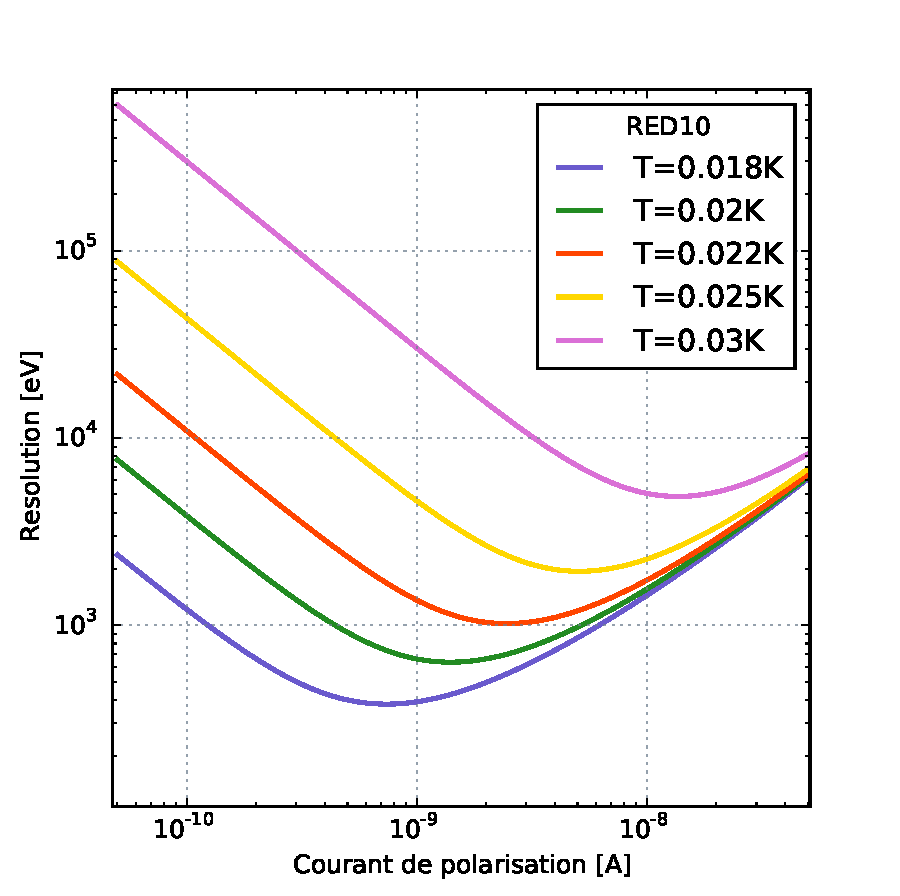
\includegraphics[width=\textwidth]{Images/red10_i.pdf}
\end{minipage}
\hfill
\begin{minipage}{0.49\textwidth}
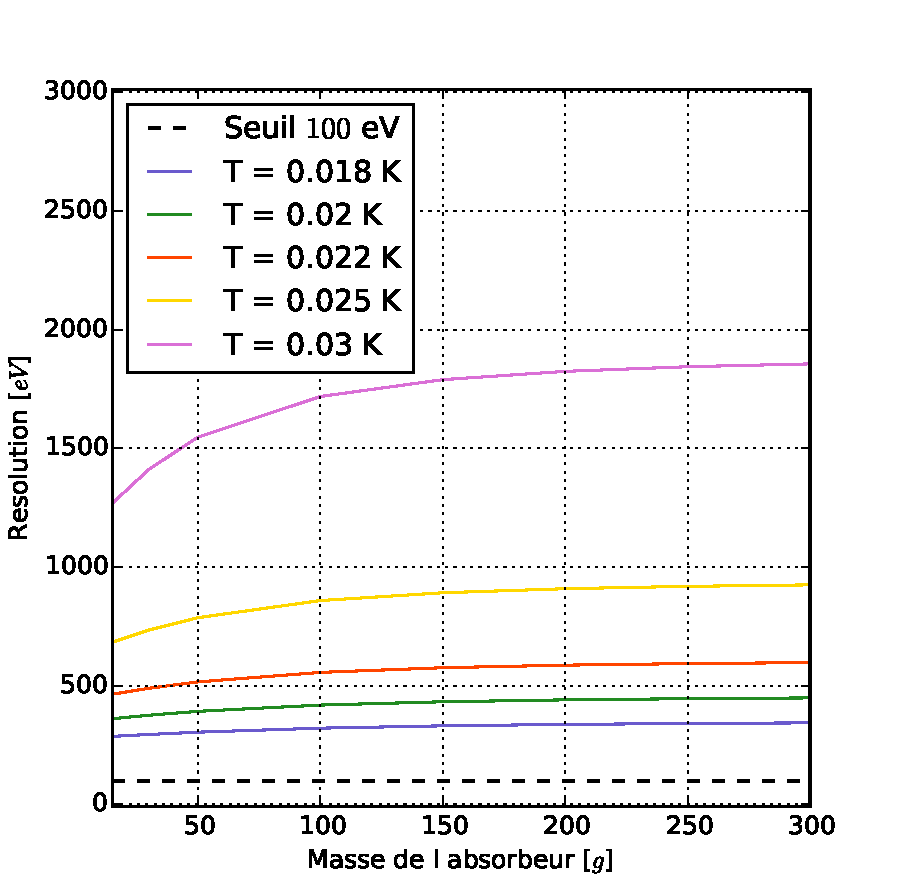
\includegraphics[width=\textwidth]{Images/red10_mass.pdf}
\end{minipage}
\caption{(à gauche) Simulation de la résolution de RED10 en fonction du courant de polarisation pour différentes températures. \\ (à droite) Simulation de la résolution à courant de polarisation optimisé en fonction de la masse de l'absorbeur pour différentes températures. Le design considéré est le même que celui de RED10, on change seulement la masse de l'absorbeur en ajustant le courant de polarisation pour obtenir la résolution la plus faible.}
\label{optim}
\end{figure}

L'étude de RED10 s'est entièrement réalisée pour un courant de polarisation de $4$nA, ce qui correspond au courant optimal d'une température d'environ $24$mK. Il aurait donc été possible d'obtenir de meilleures valeurs de résolution en ajustant pour chaque température le courant de polarisation. Ainsi, il sera important, dans le futur, de bien déterminé le courant de polarisation optimum d'un détecteur suivant les conditions de mesures.

La recherche de matière noire légère nécessite de mettre au point une nouvelle génération de détecteur avec de très bas seuil de détection. Pour cela, il est nécessaire de travailler sur le design des détecteurs. Il faut par exemple étudier le comportement du détecteur selon la géométrie du NTD, la masse de l'absorbeur ou encore l'emplacement des fuites thermiques. On présente sur le graphe à droite de la figure \ref{optim}, une simulation de la résolution d'un détecteur en fonction de la masse de l'absorbeur. On notera que le courant de polarisation est ajusté pour chaque point afin de tracer une courbe de résolution déjà optimisée. D'après la formule (\ref{capa}), il serait intéressant de réduire la capacité thermique de l'absorbeur $C$, en abaissant sa masse, afin de provoquer une plus grande élévation en température $\Delta T$, et ainsi amplifier le signal chaleur. D'après la simulation, cette amplification du signal chaleur n'apparaîtrait que pour de très petites masses de détecteur, et resterait très modeste pour les faibles températures. 

On comprend maintenant qu'on reste limité pour le moment par un autre aspect du détecteur. Dans le futur, l'optimisation du détecteur va passer par l'étude du comportement en fonction des dimensions du la thermistance NTD et des surfaces de conduction thermiques. Il apparaît déjà qu'il faudrait réduire les capacités thermiques des différents bains tout en maximisant les liens thermiques. 

